\chapter{Signal Region Distributions with MC Simulation}
\label{chap:SRMC}

Distributions of various variables in \ac{SR}, which are used in the \ac{BDT} training. More details on these input features are described in \autoref{sec:Input}. The data are shown as filled points and the \ac{SM} background predictions as histograms. The VV(V) background includes ZZ and triboson production, while the $\ttbar$ + X(X) component includes $\ttbar$W, $\ttbar$Z, $\ttbar$H, tZq, and smaller backgrounds containing one or two top quarks plus a boson or quark. All backgrounds are estimated using \ac{MC} simulation. The hatched bands indicate statistical and systematic uncertainties for the \ac{SM} background predictions. The normalisation of the signal processes is chosen arbitrarily for improved visualisation. 

\begin{figure}[tbh!]
 \begin{center}
 \begin{tabular}{ccc}
    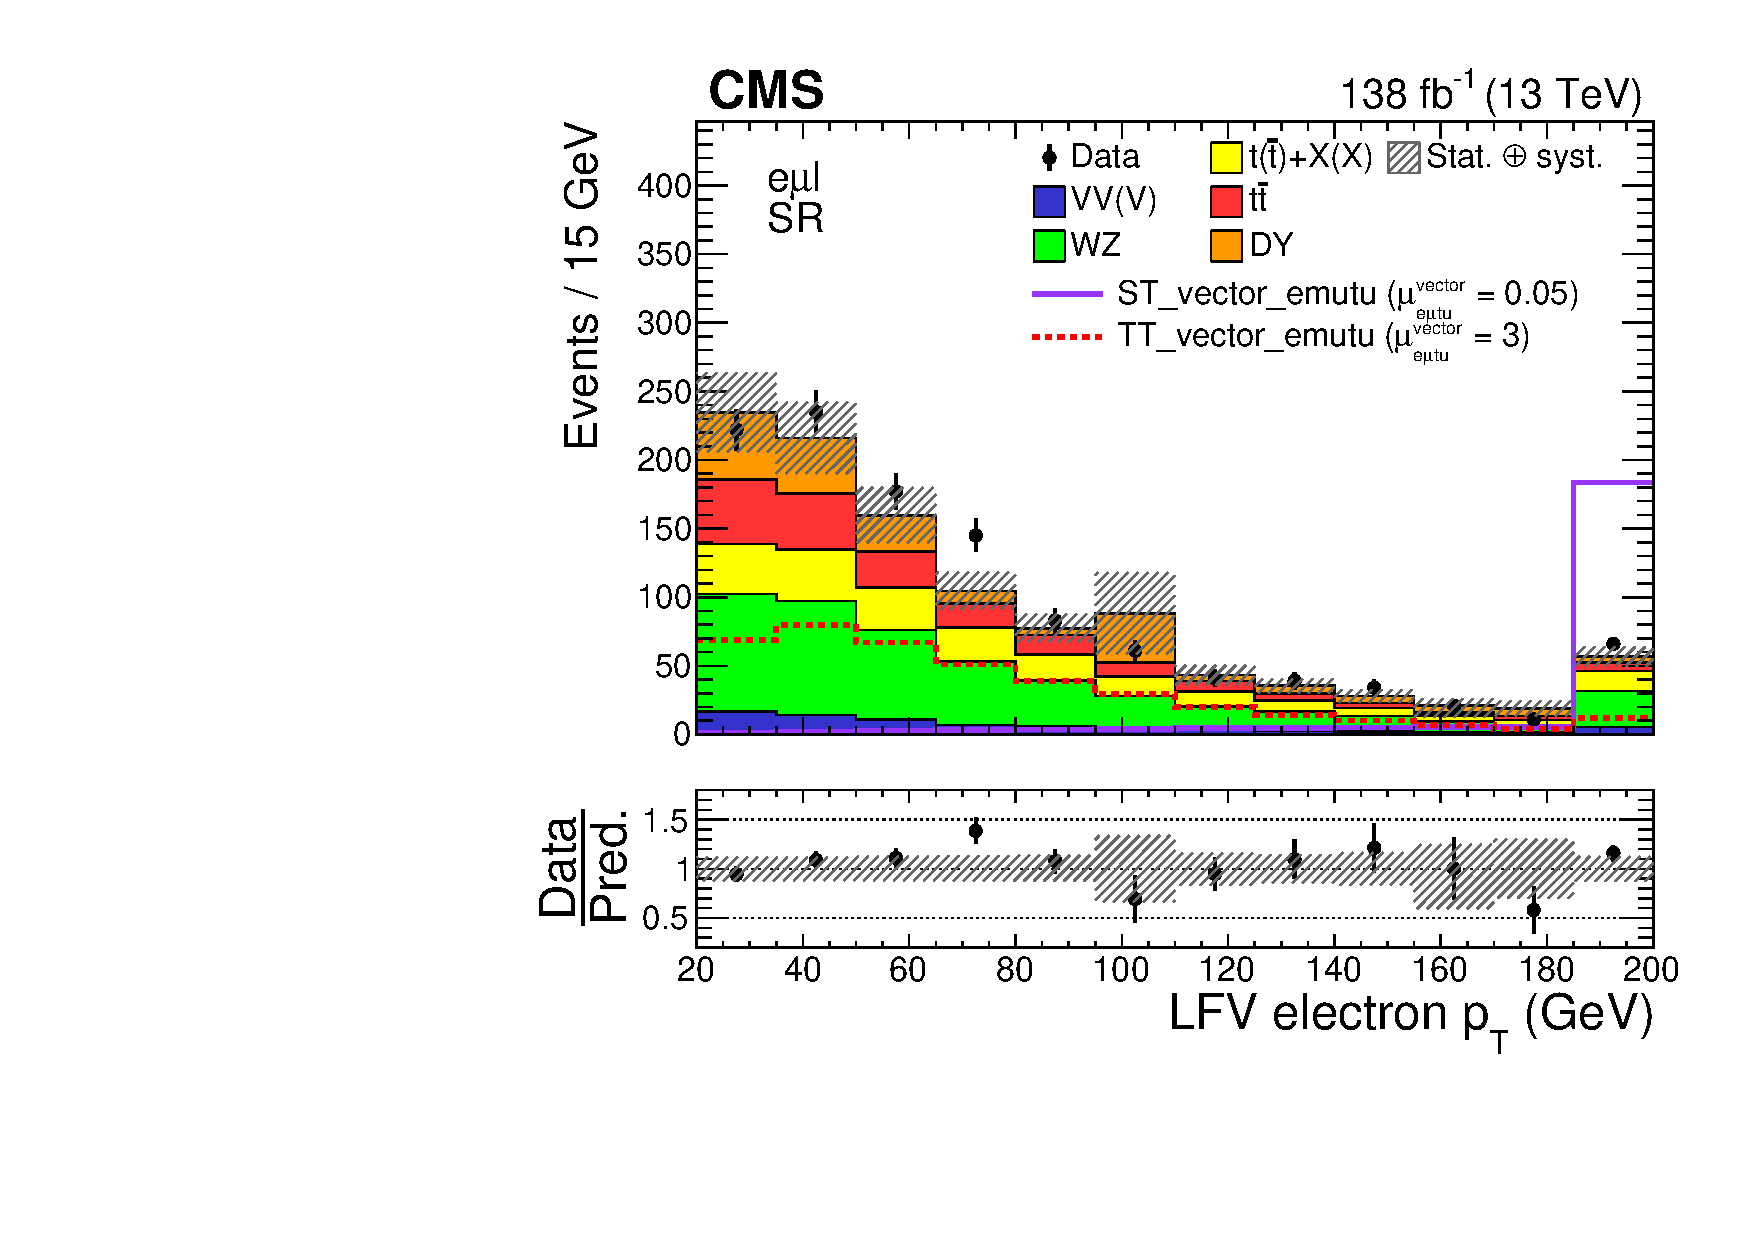
\includegraphics[width=0.325\textwidth]{figures/Appendix/SRMC/LFVePt}&
    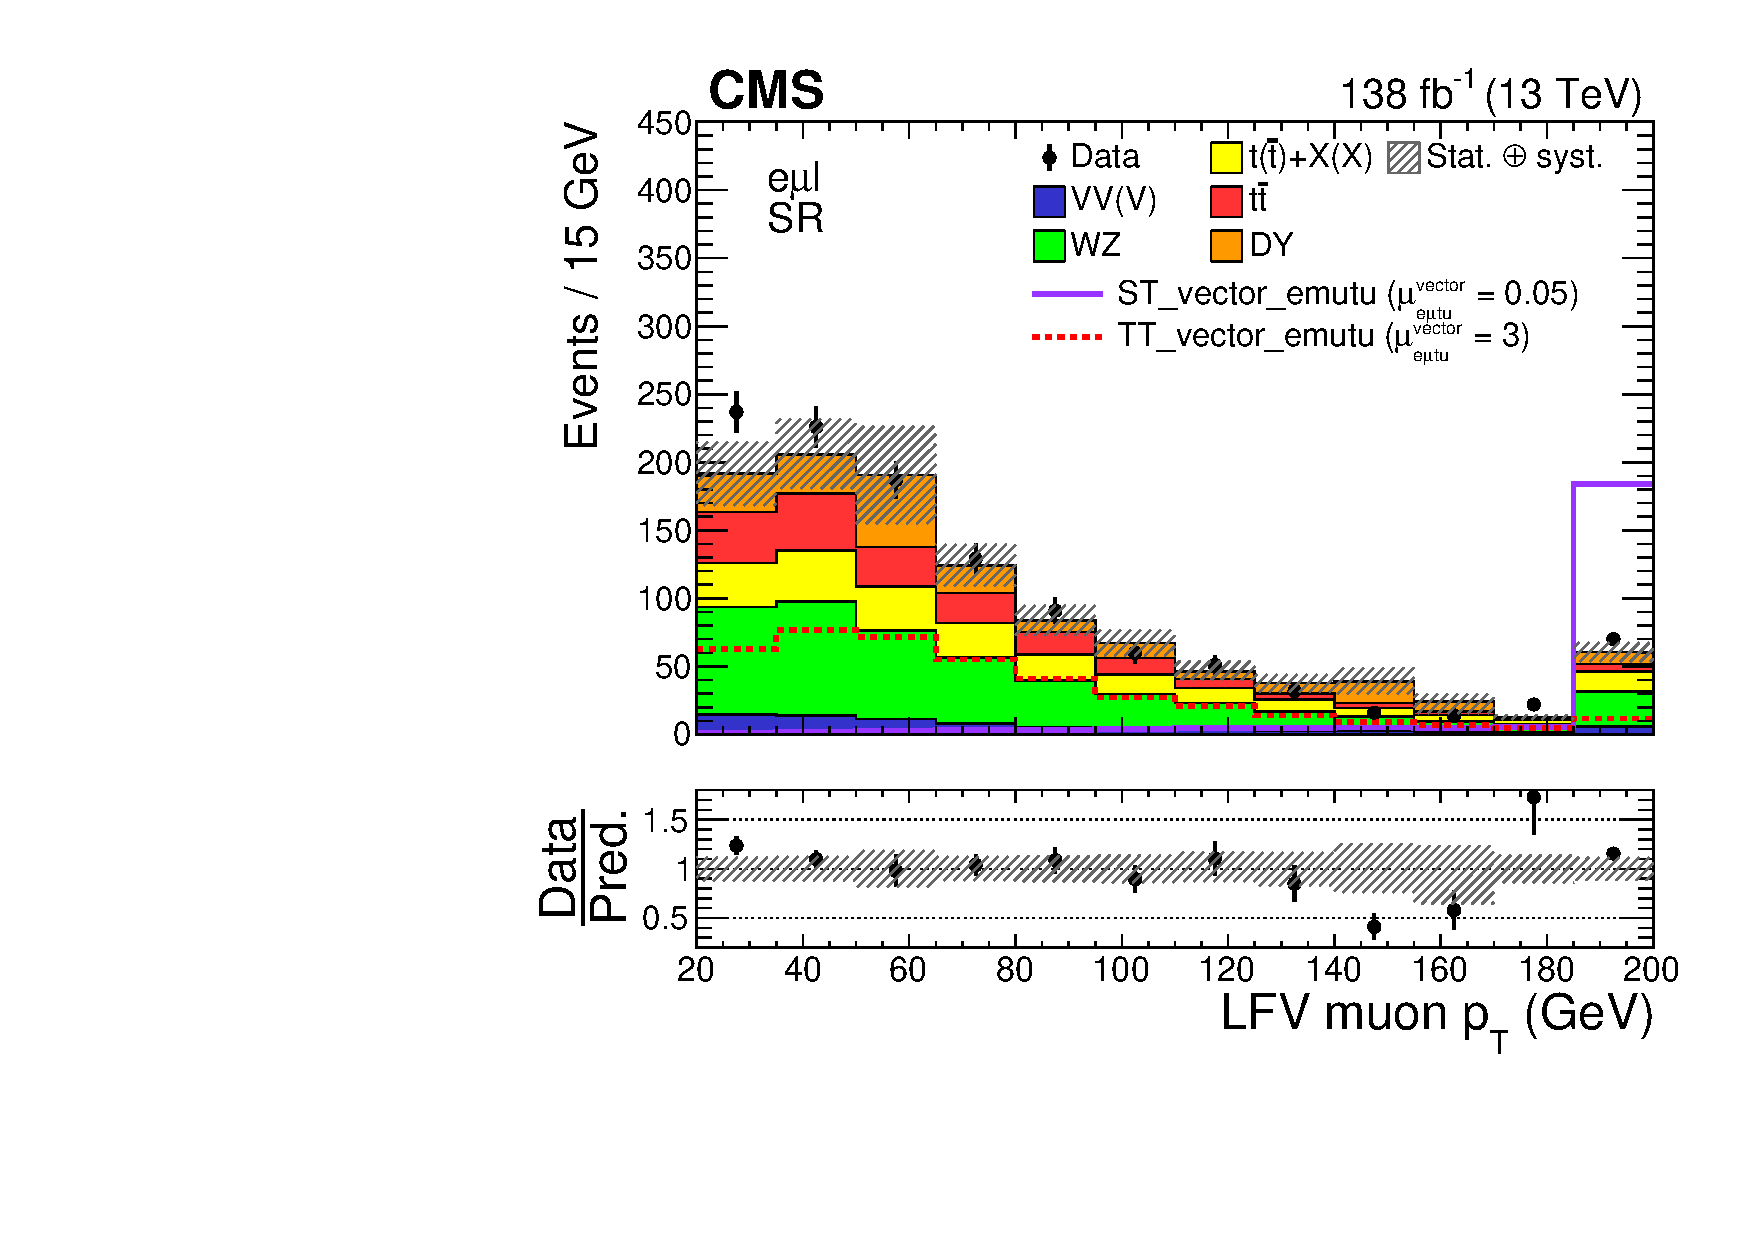
\includegraphics[width=0.325\textwidth]{figures/Appendix/SRMC/LFVmuPt}&
    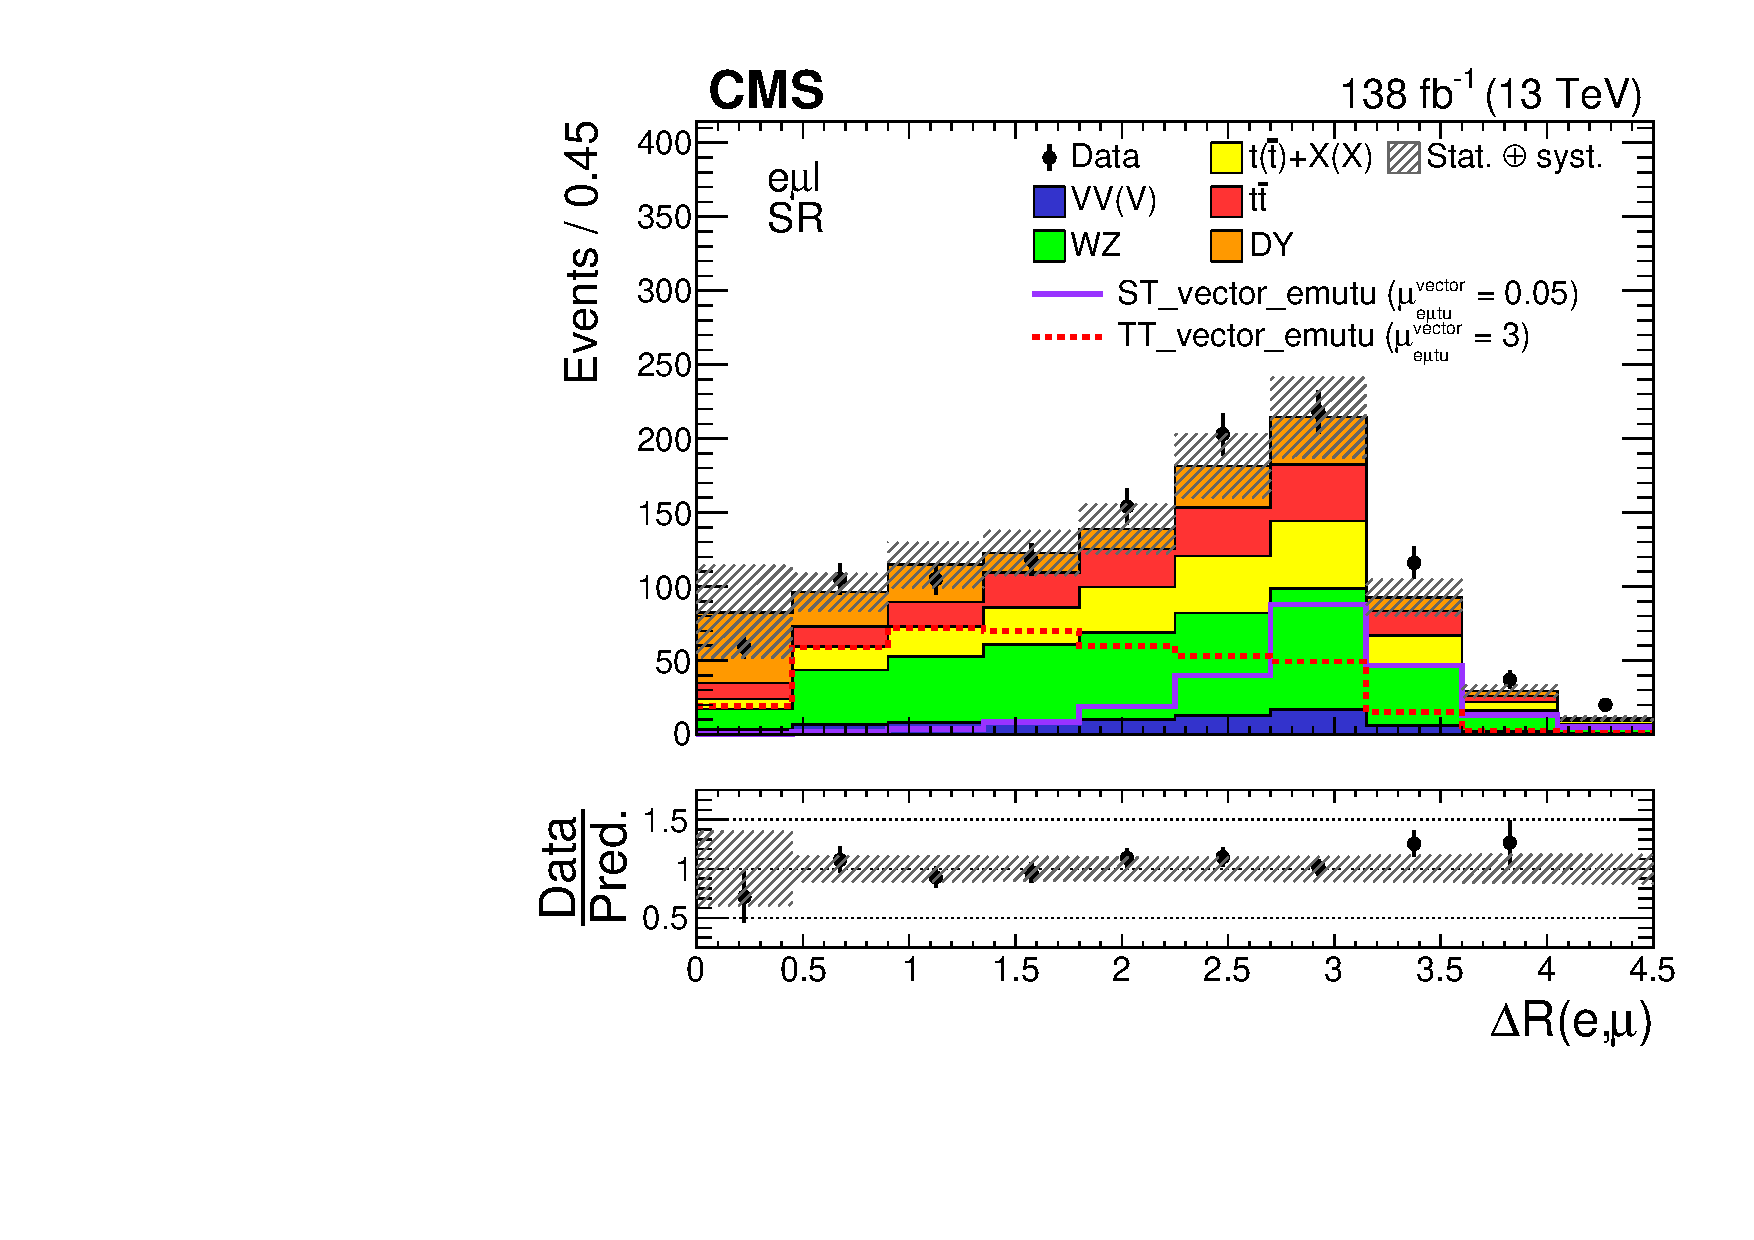
\includegraphics[width=0.325\textwidth]{figures/Appendix/SRMC/llDr}\\
 \end{tabular}
 \caption{Distributions of LFV electron $\pt$ (left), LFV muon $\pt$ (middle), and the opening angle between LFV electron and LFV muon (right).}
 \label{fig:input_vali_1}
 \end{center}
\end{figure}

\begin{figure}[tbh!]
 \begin{center}
 \begin{tabular}{ccc}
  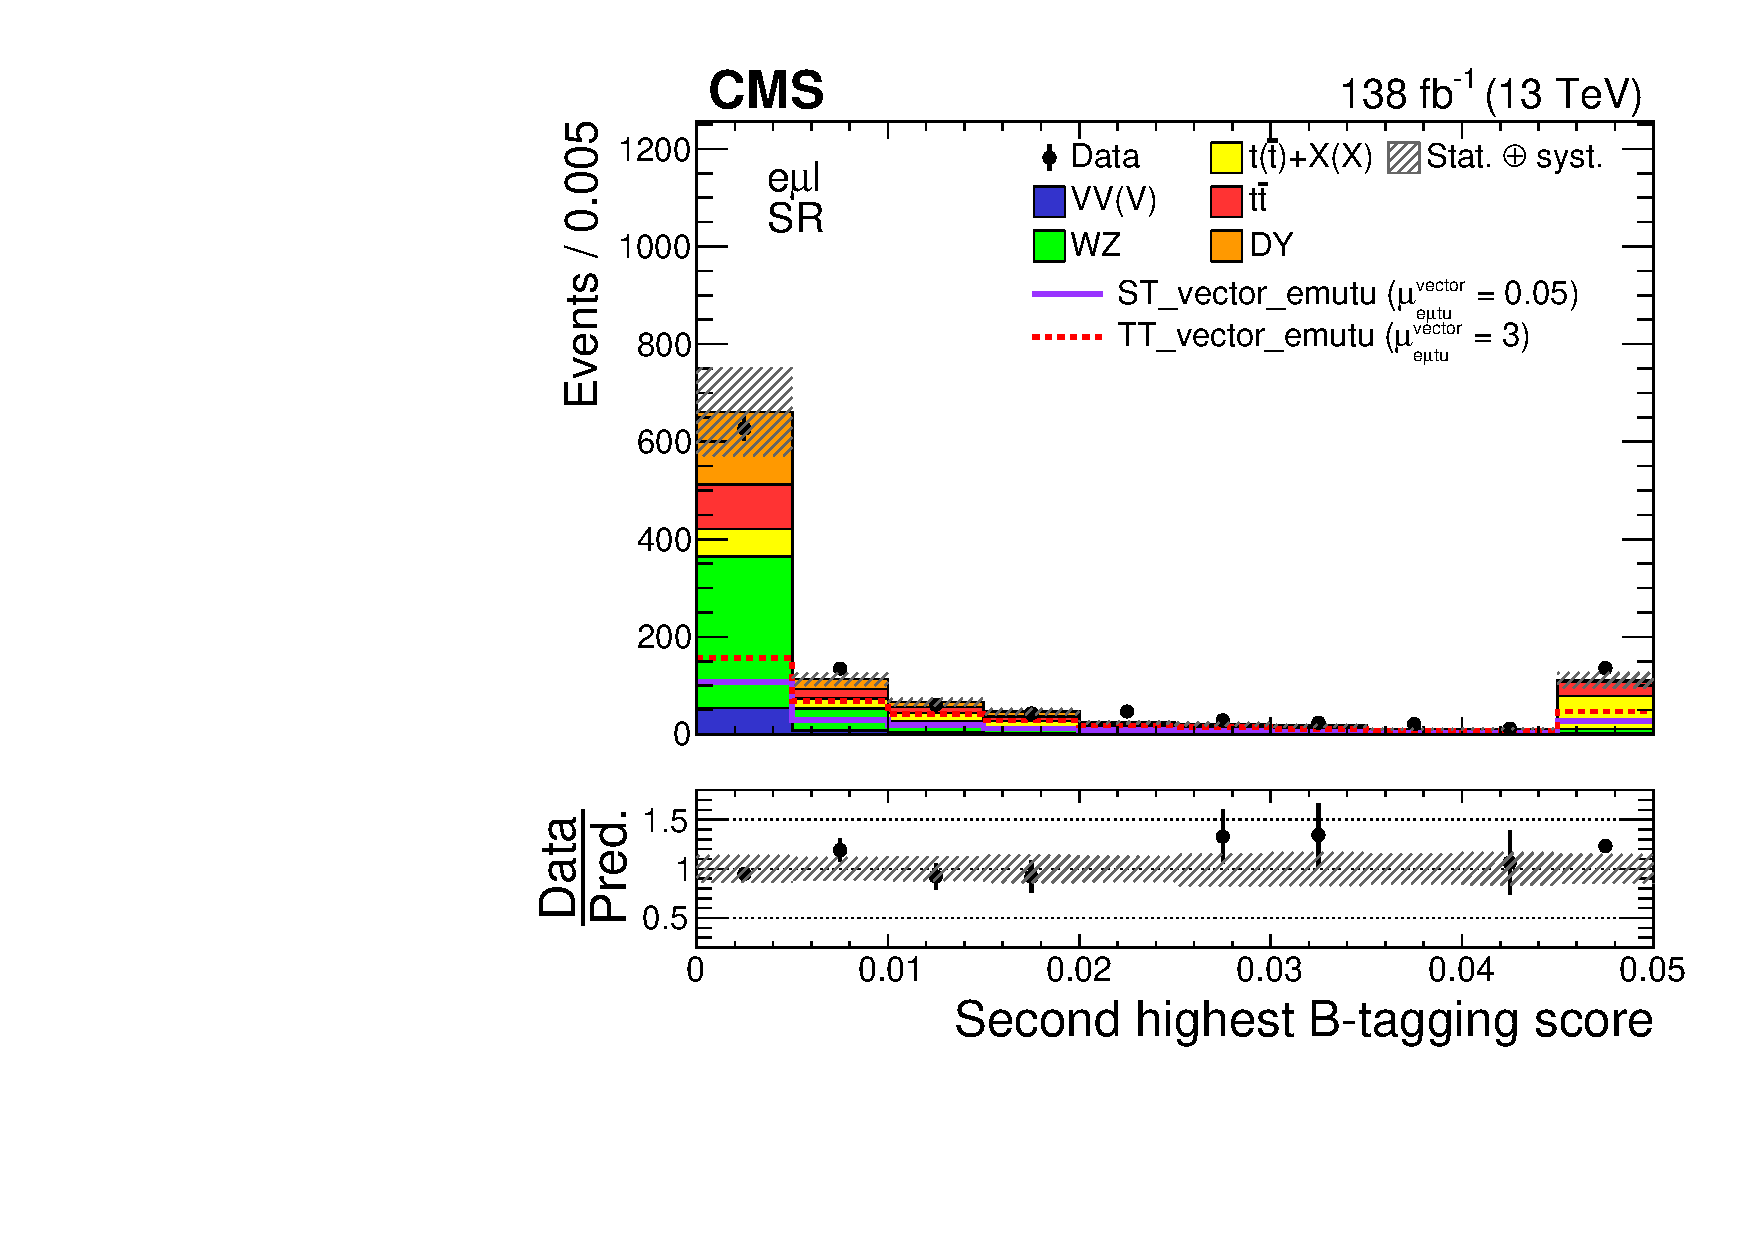
\includegraphics[width=0.325\textwidth]{figures/Appendix/SRMC/Jet2Btag}&
  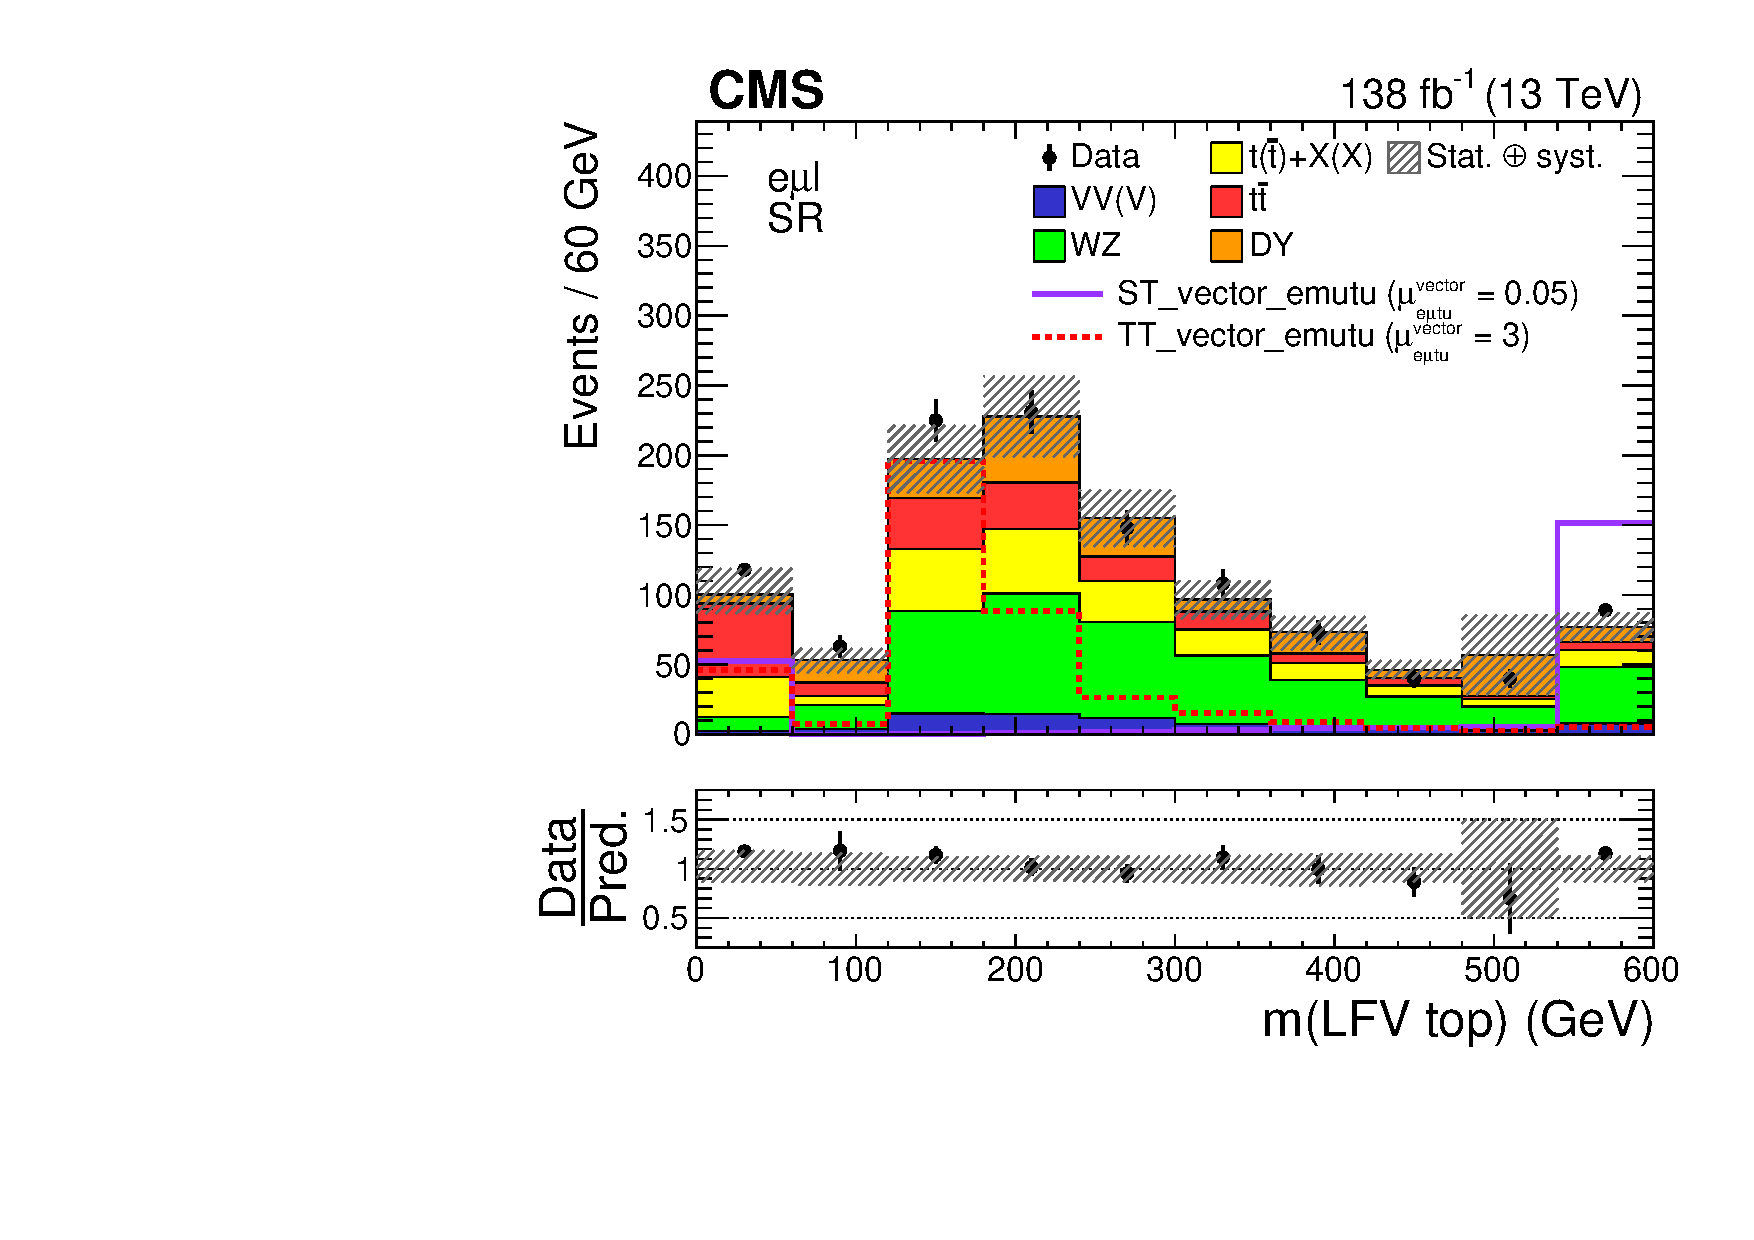
\includegraphics[width=0.325\textwidth]{figures/Appendix/SRMC/LFVTopmass}&
  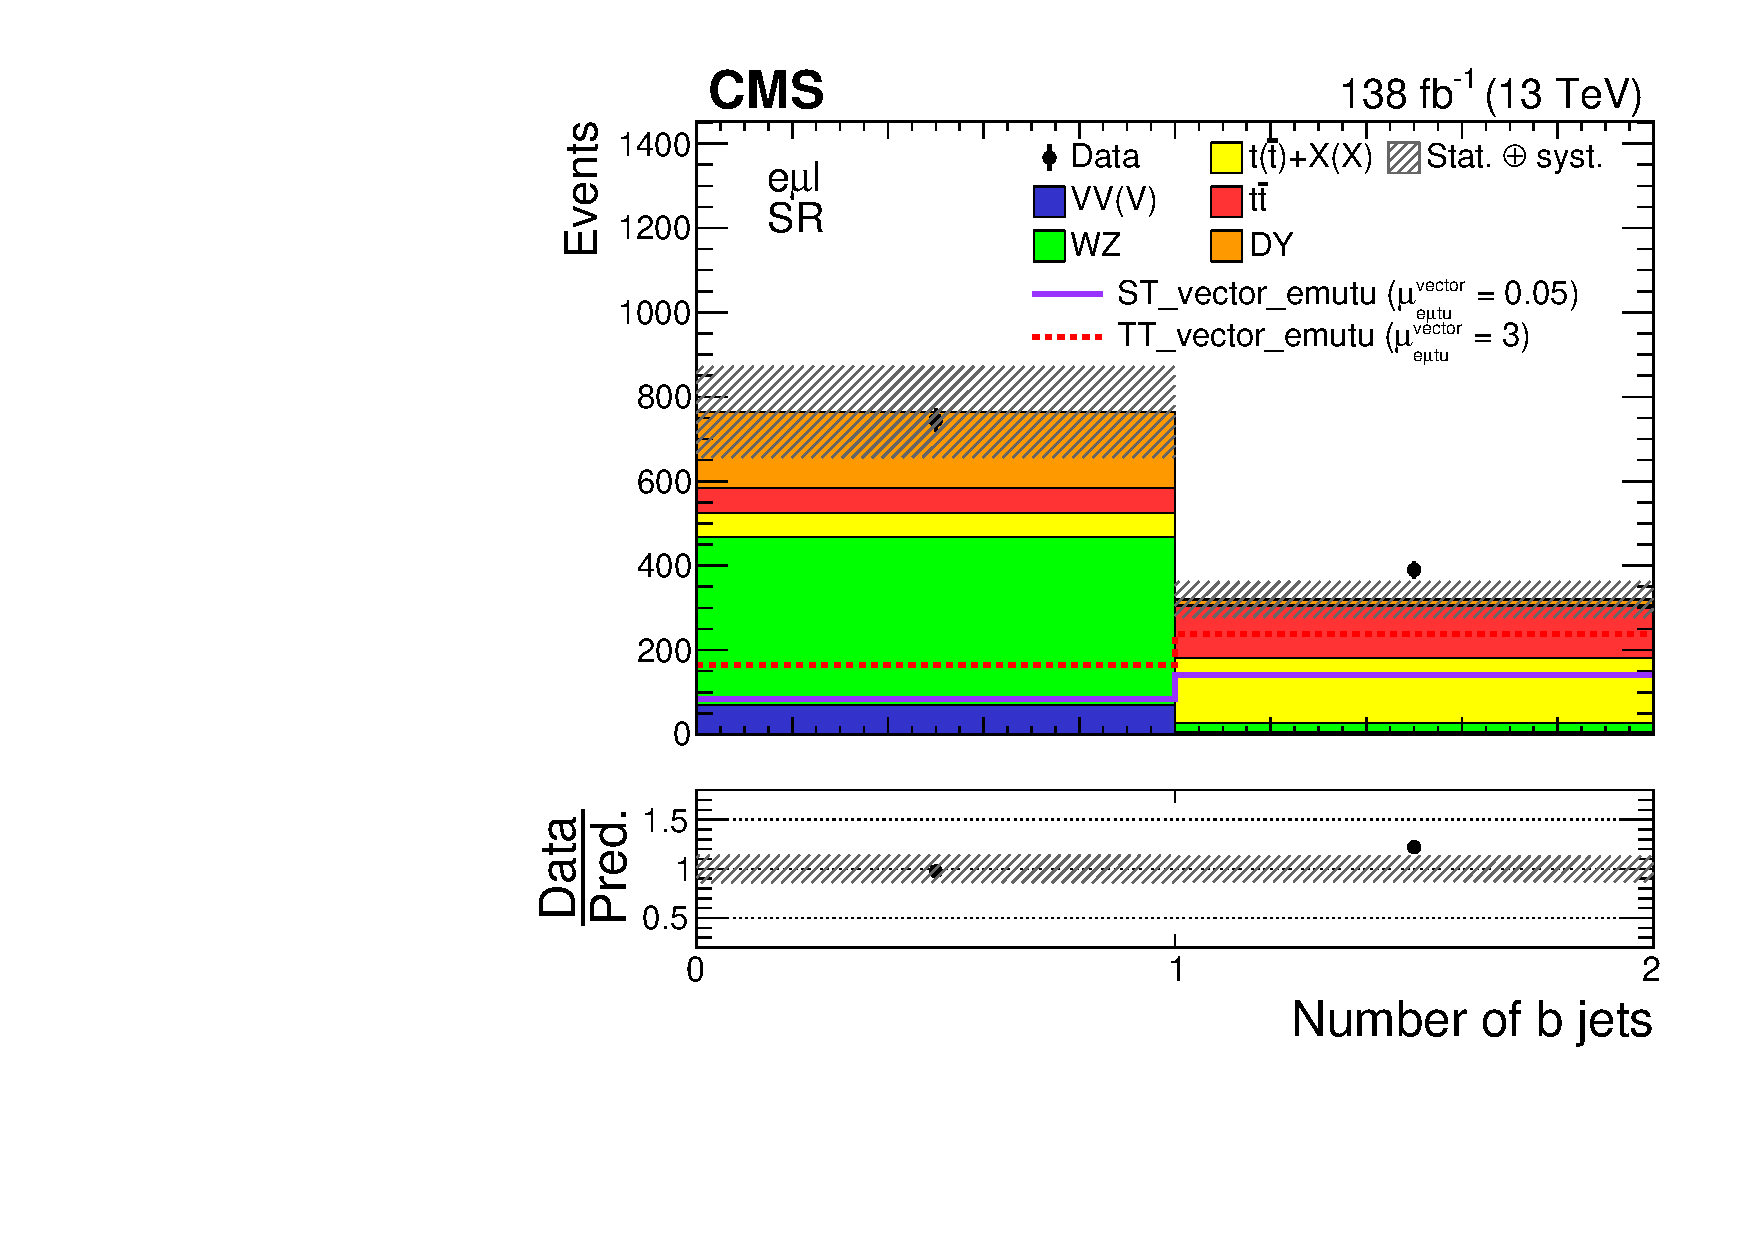
\includegraphics[width=0.325\textwidth]{figures/Appendix/SRMC/nbjet}\\
 \end{tabular}
 \caption{Distributions of the second highest \DeepJ score (left), LFV top mass (middle), b jet multiplicity (right).}
 \label{fig:input_vali_2}
 \end{center}
\end{figure}

\begin{figure}[tbh!]
 \begin{center}
 \begin{tabular}{ccc}
  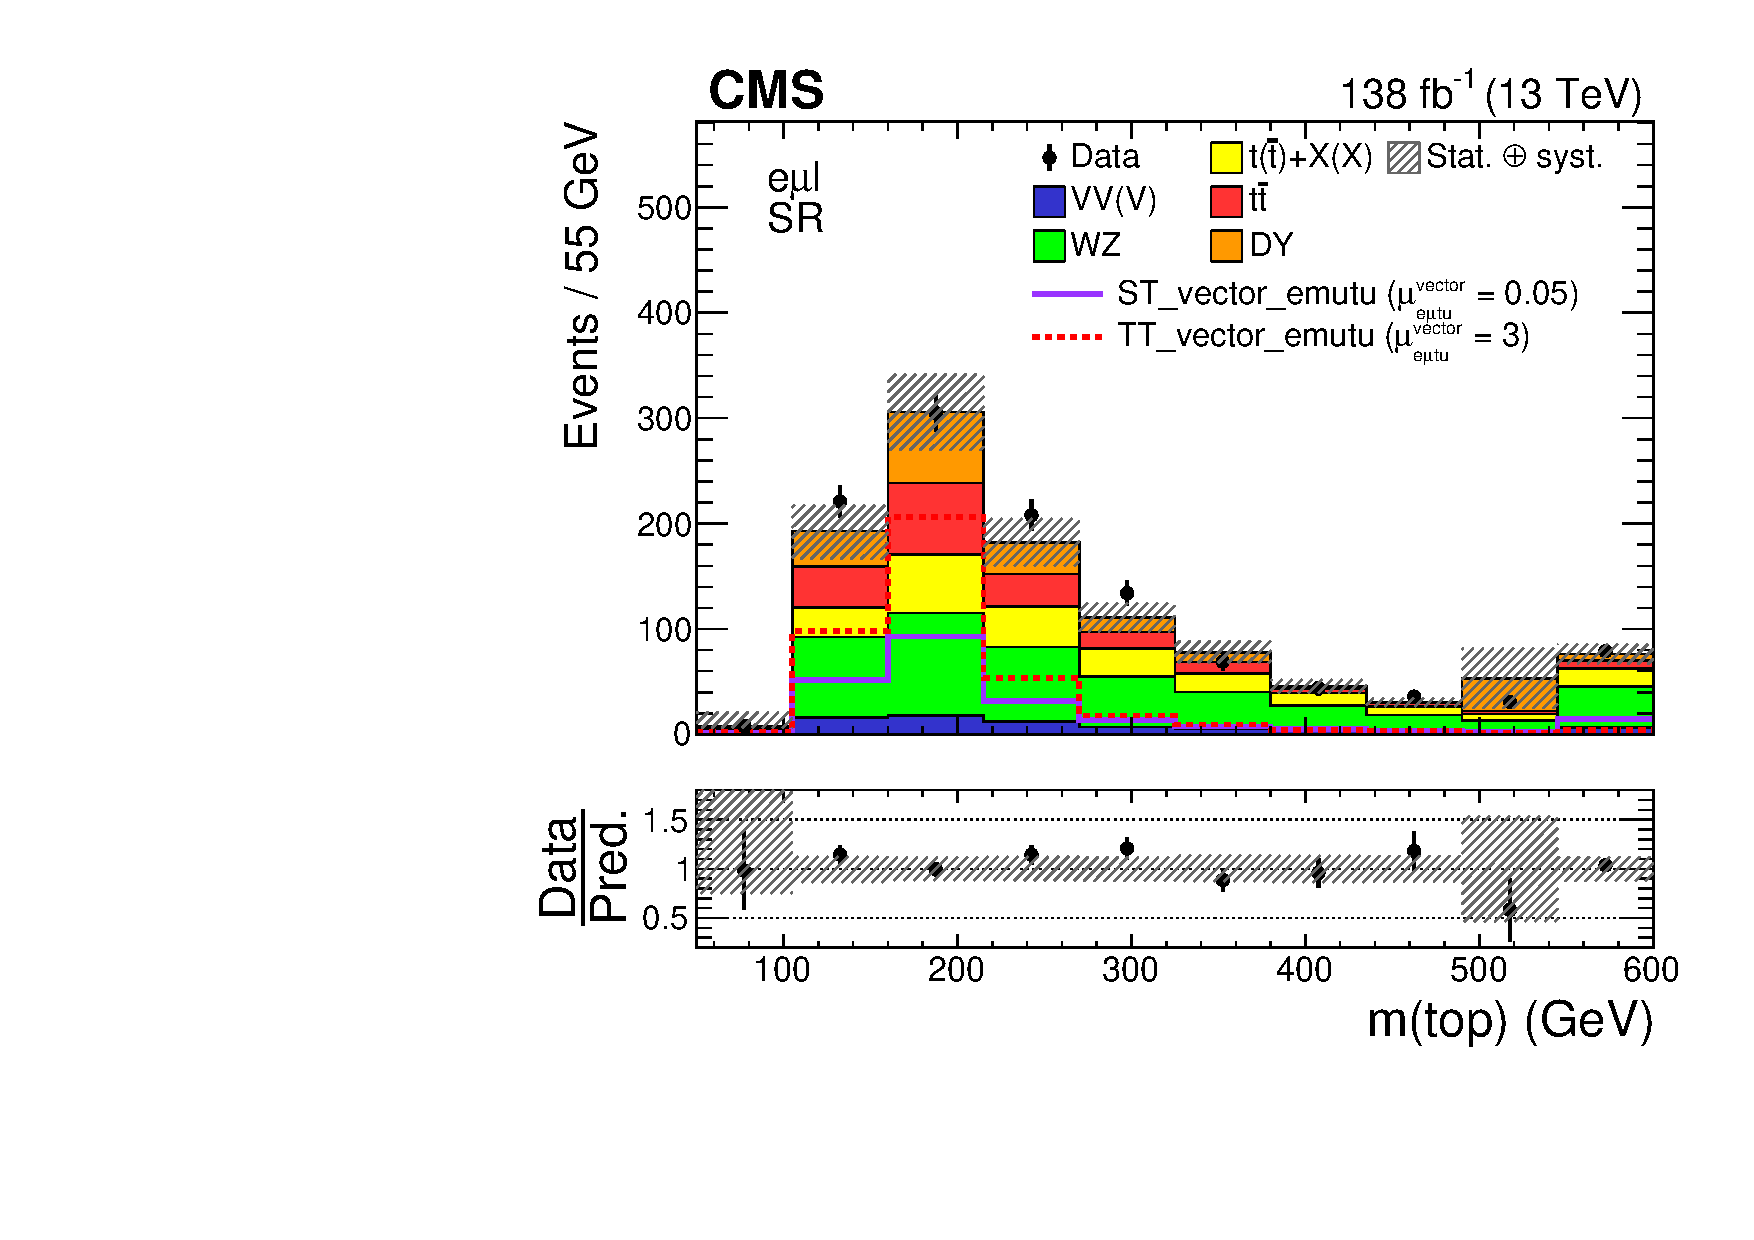
\includegraphics[width=0.325\textwidth]{figures/Appendix/SRMC/Topmass}&
    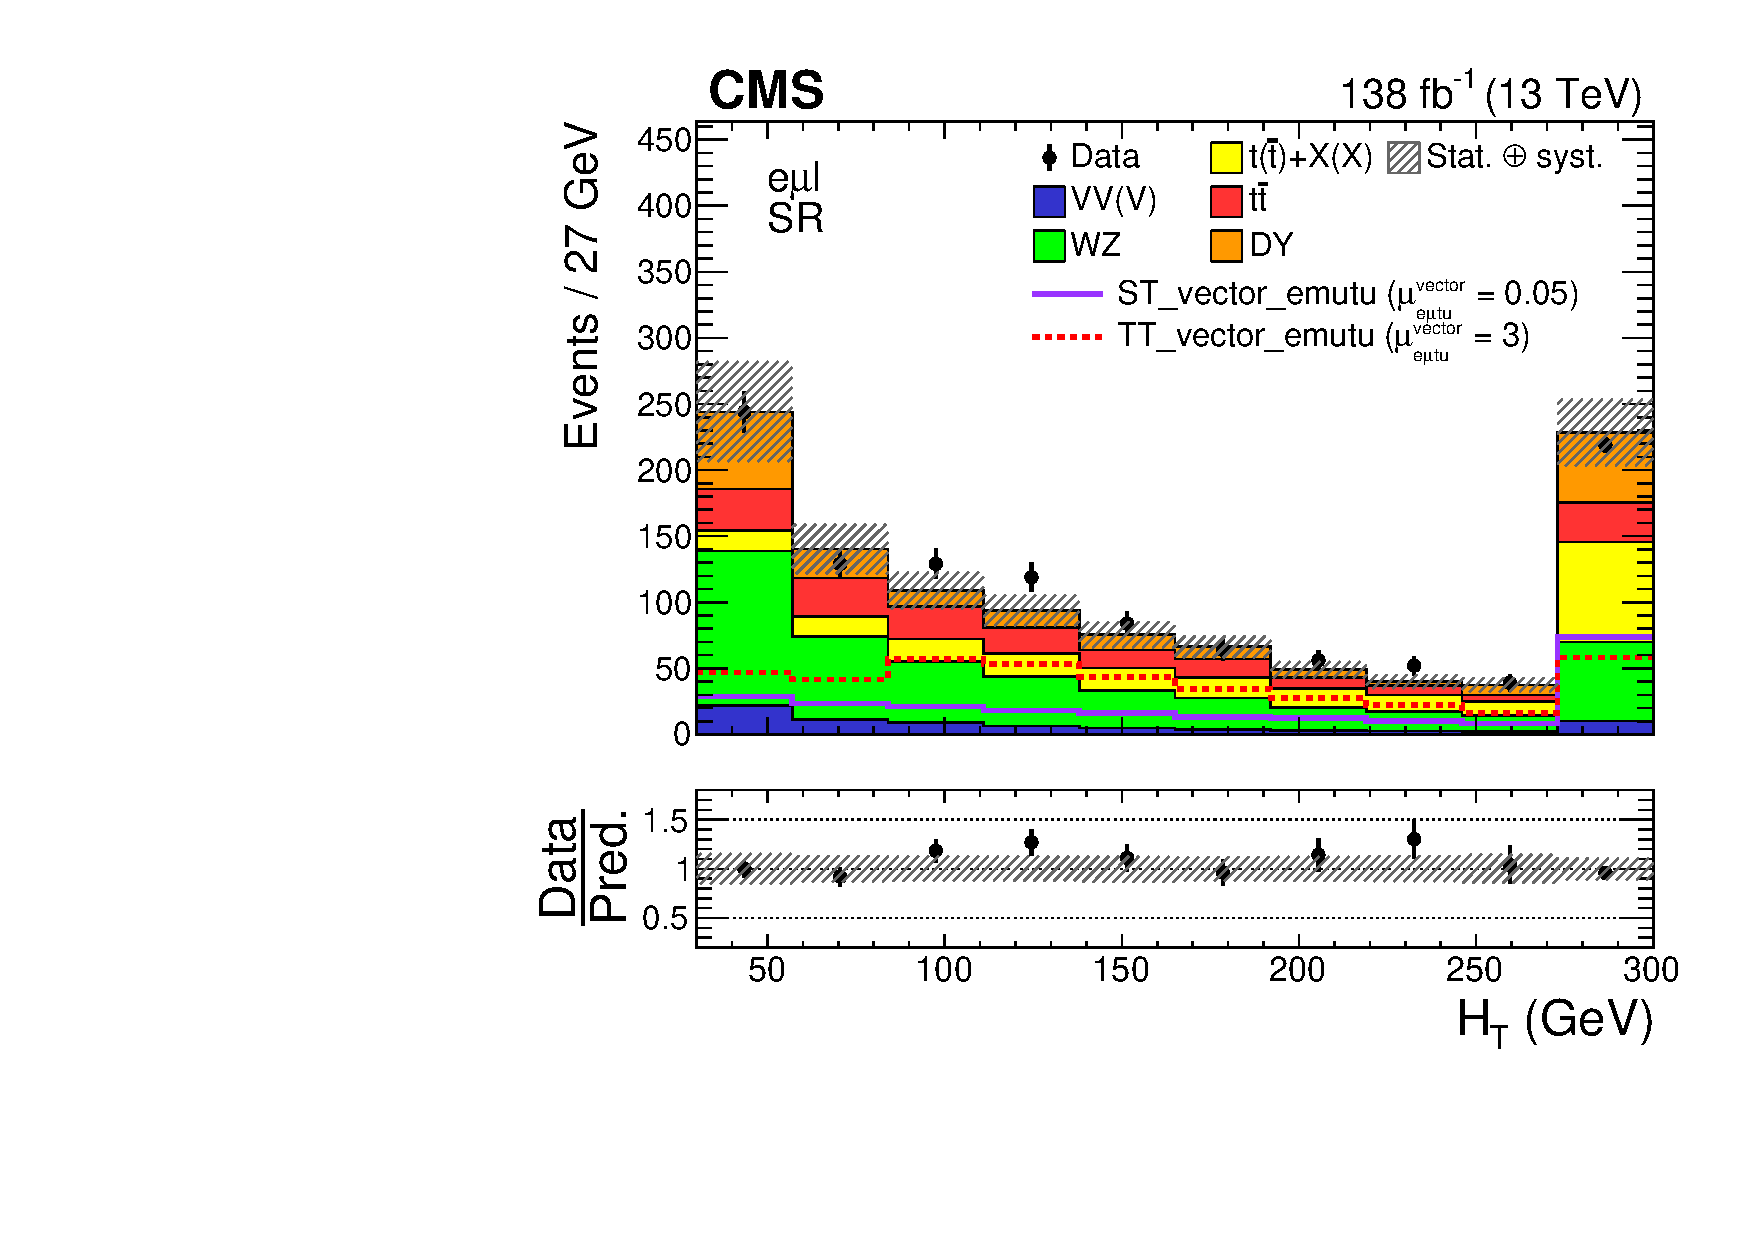
\includegraphics[width=0.325\textwidth]{figures/Appendix/SRMC/JetHt}&
  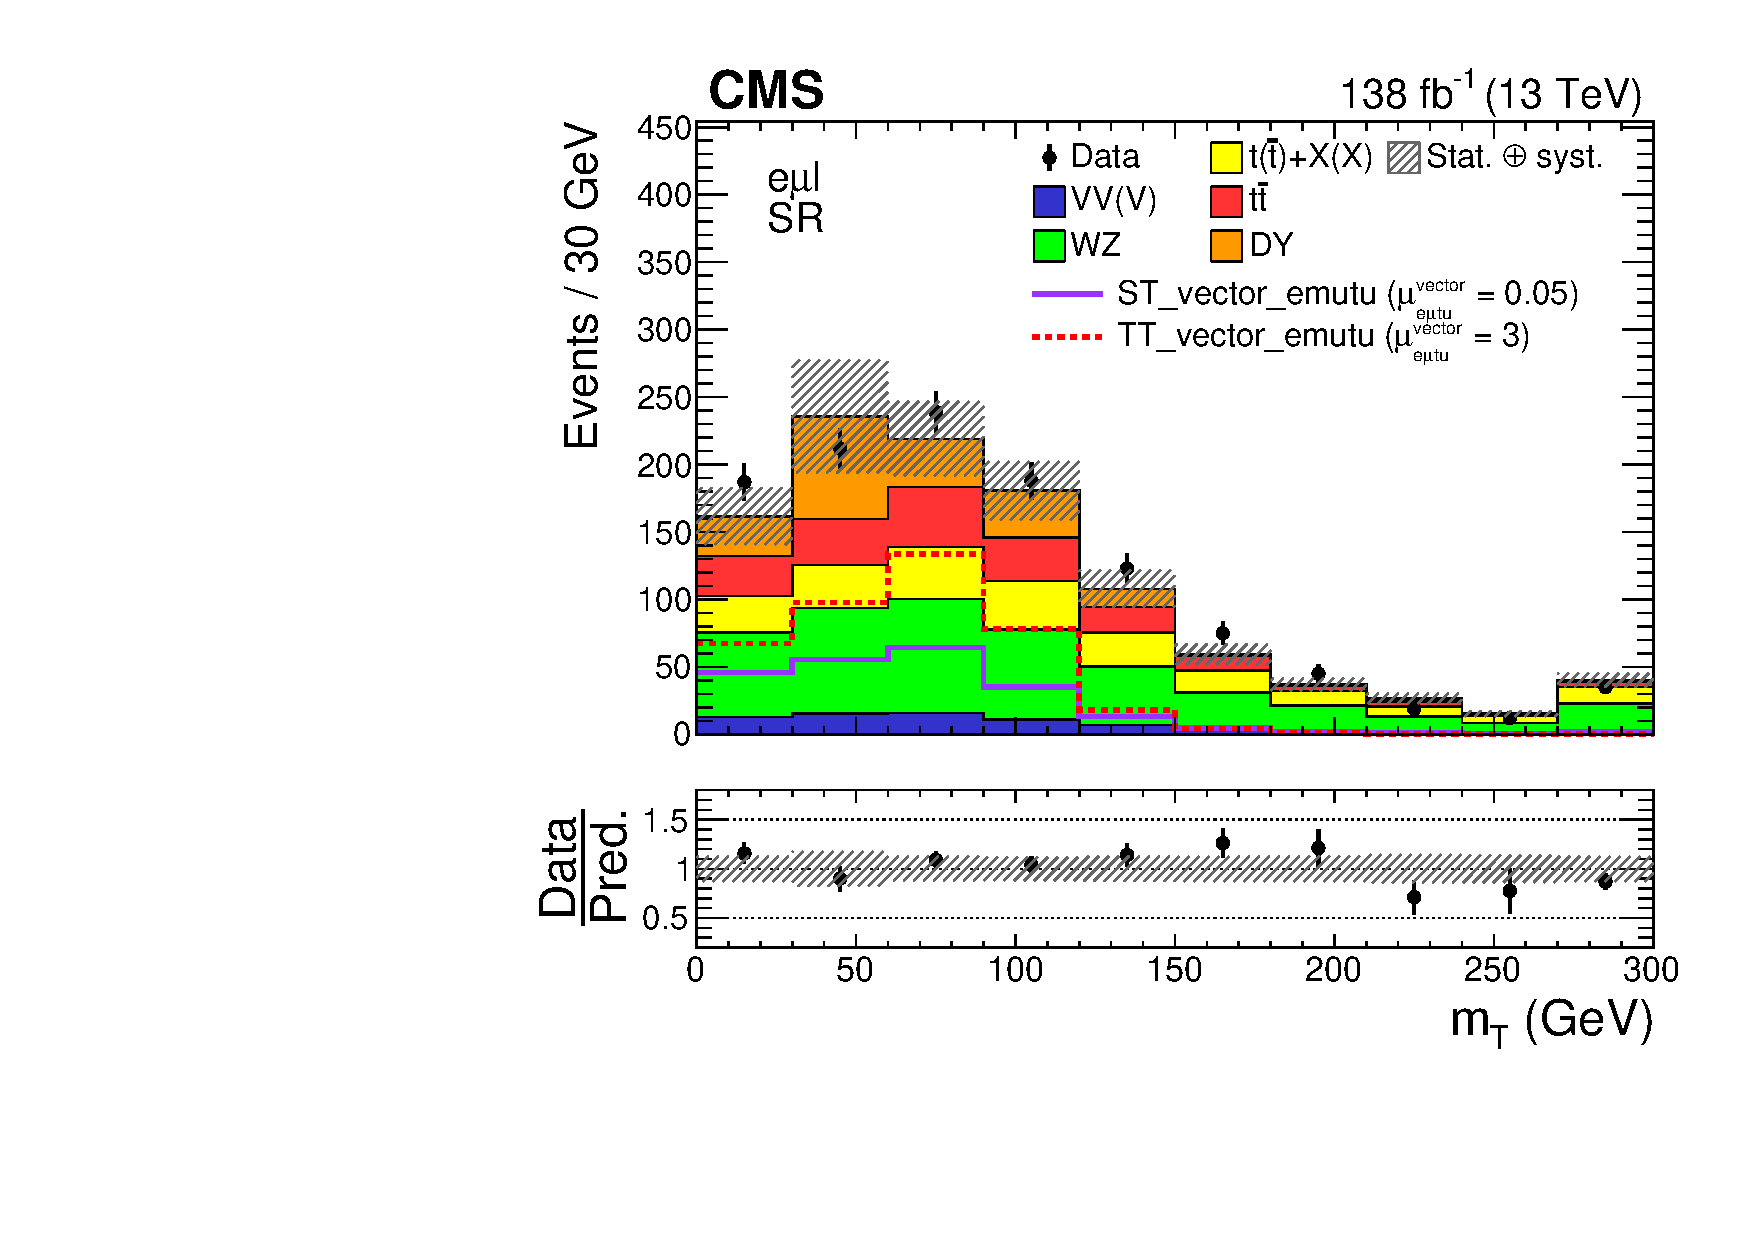
\includegraphics[width=0.325\textwidth]{figures/Appendix/SRMC/tM}\\
 \end{tabular}
 \caption{Distributions of \ac{SM} top quark mass (left), scalar sum of $\pt$ of all jets (middle), and transverse mass of the W boson (right).}
 \label{fig:input_vali_3}
 \end{center}
\end{figure}

\begin{figure}[tbh!]
 \begin{center}
 \begin{tabular}{ccc}
  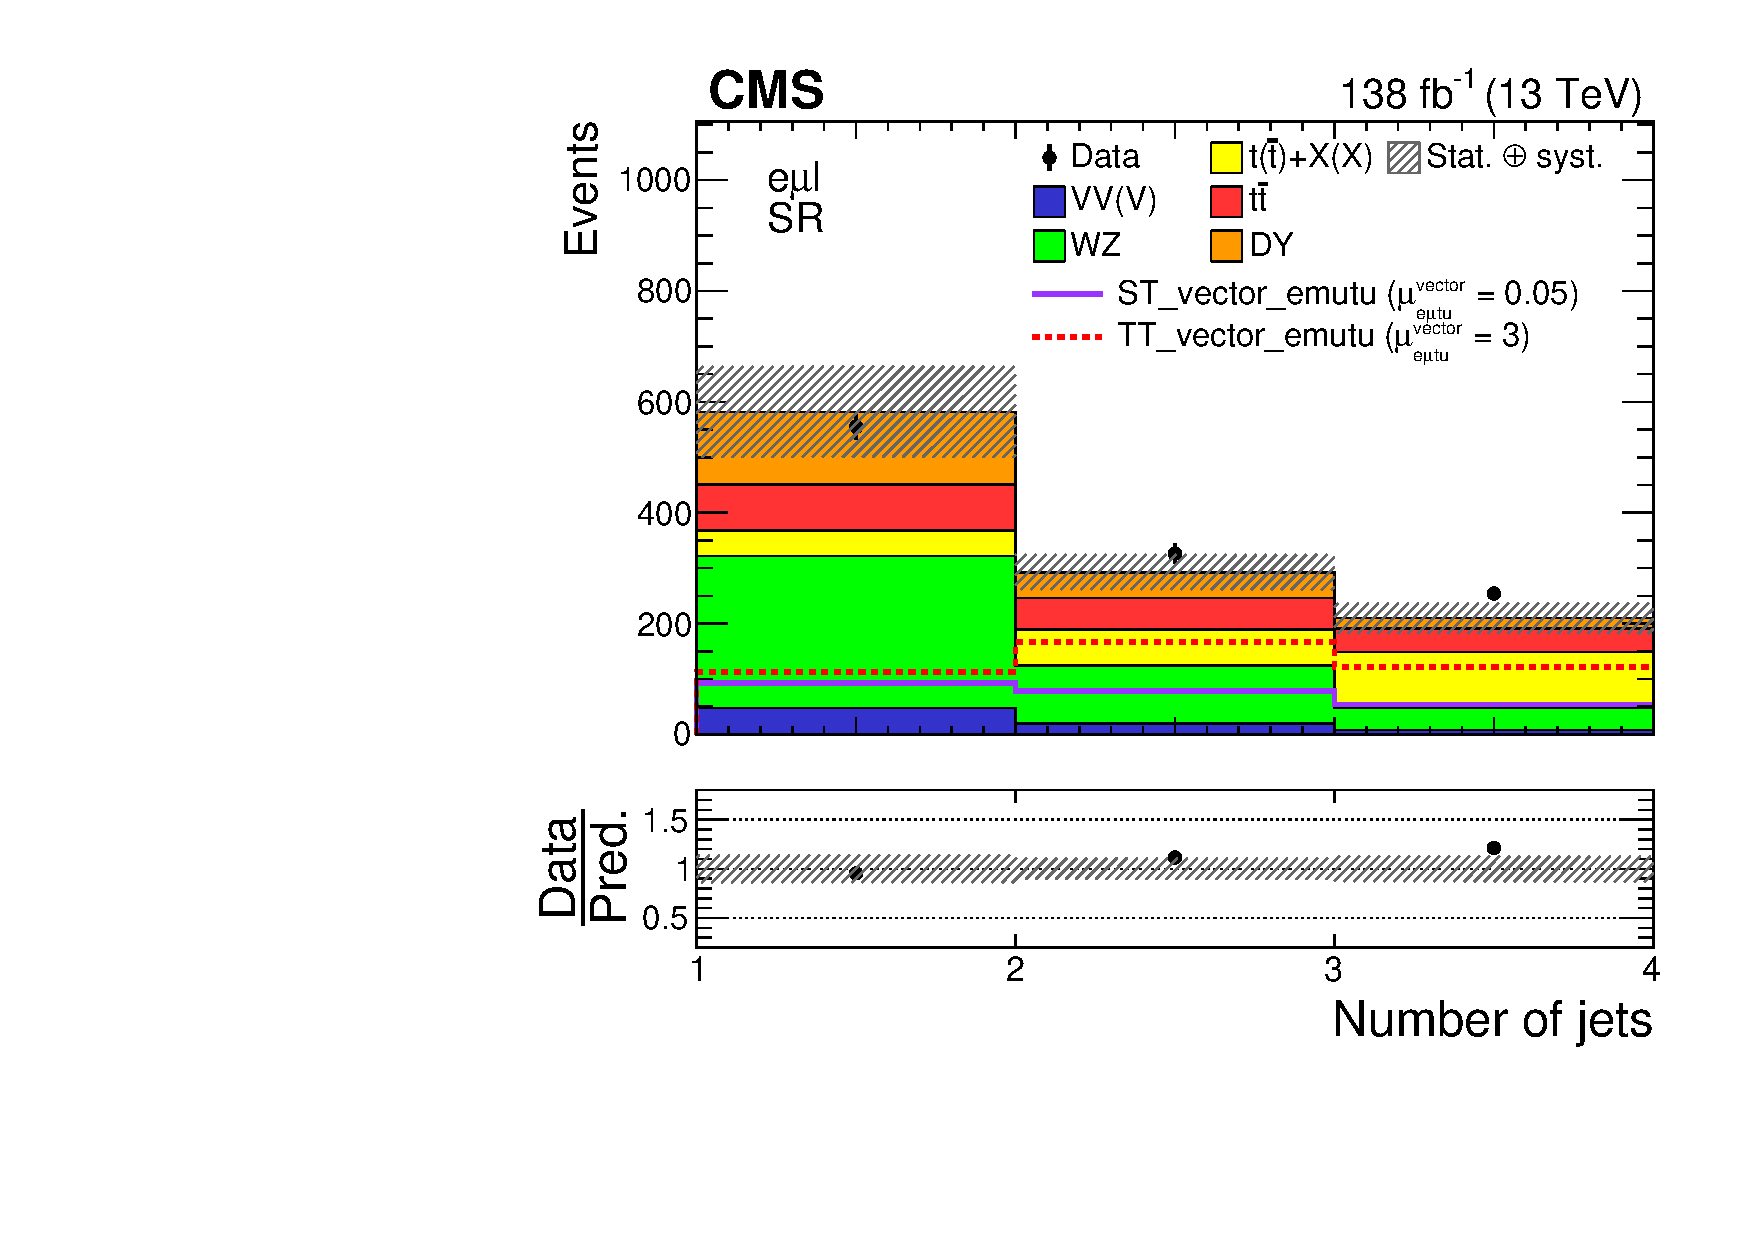
\includegraphics[width=0.325\textwidth]{figures/Appendix/SRMC/njet}&
    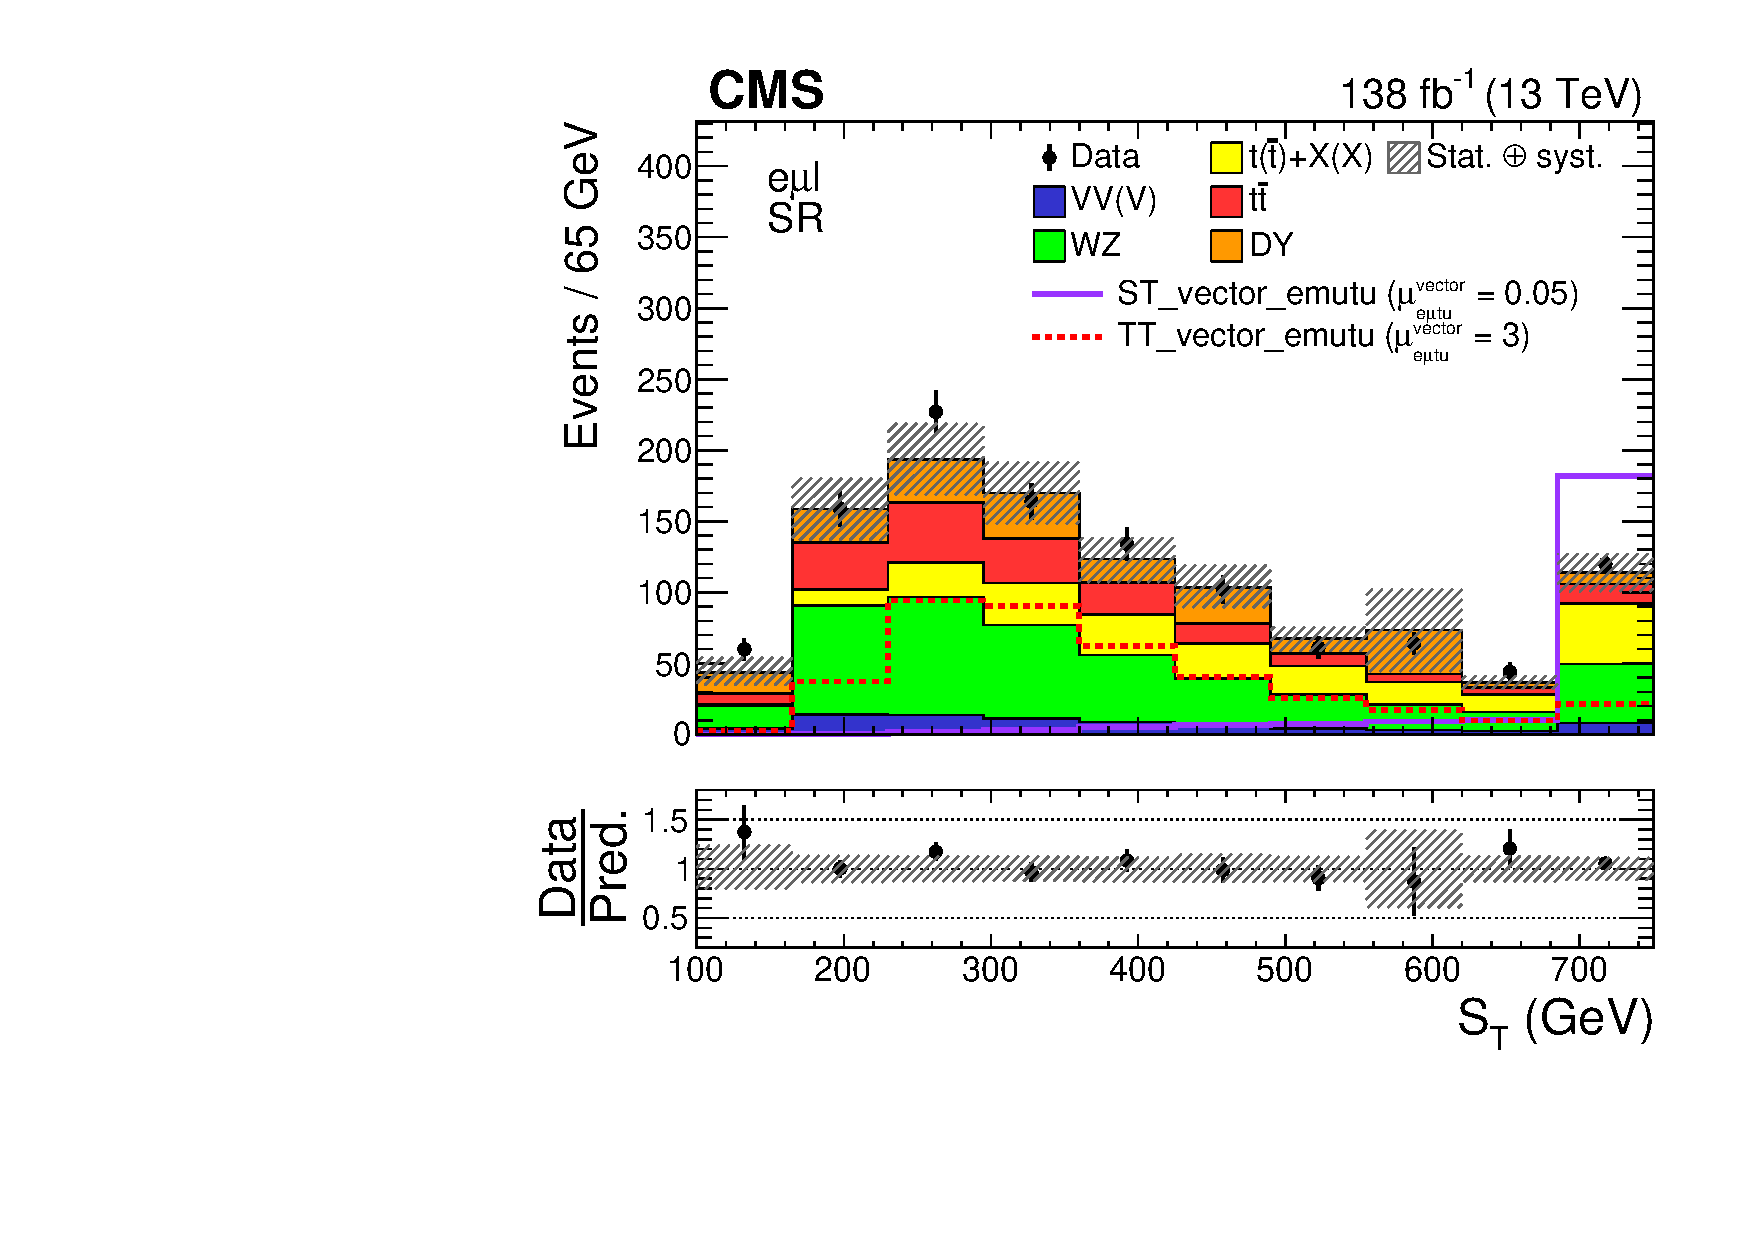
\includegraphics[width=0.325\textwidth]{figures/Appendix/SRMC/Ht}&
  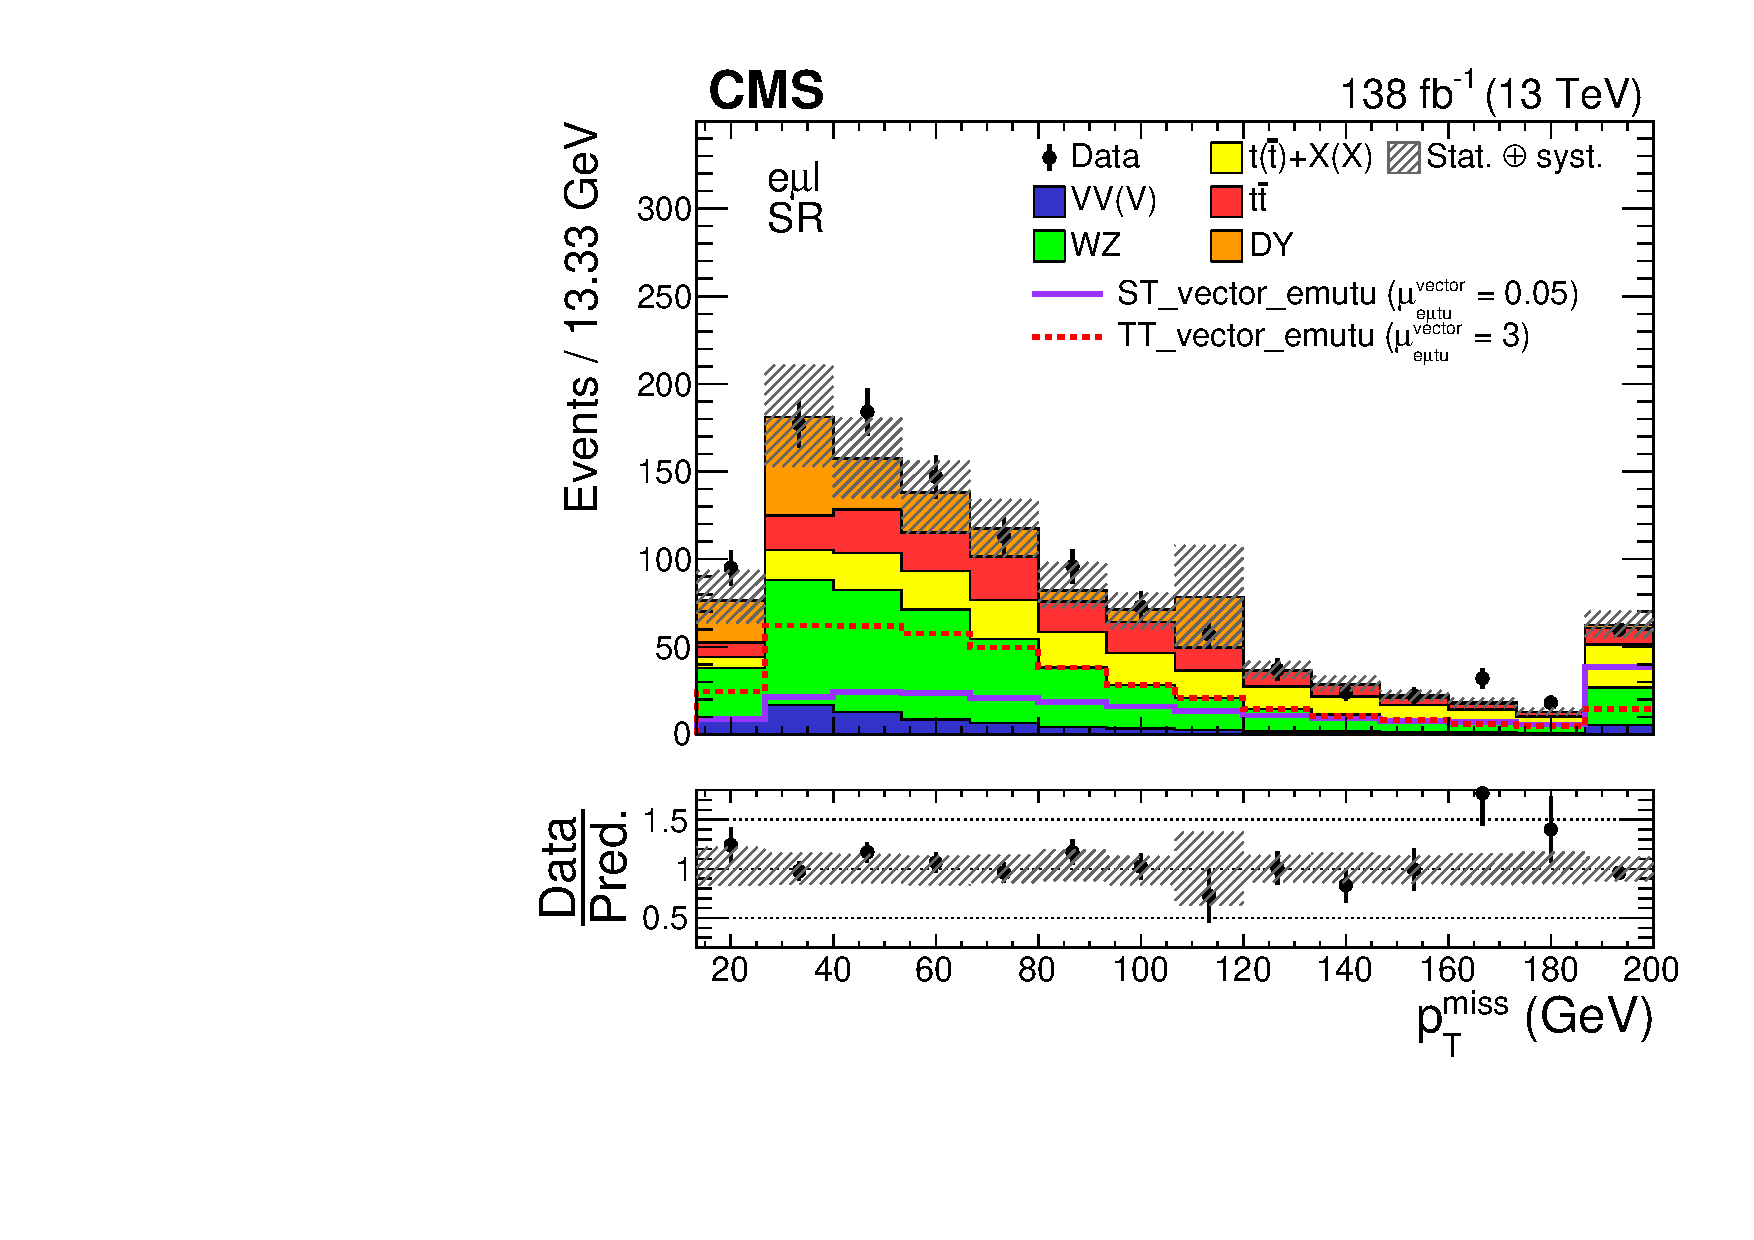
\includegraphics[width=0.325\textwidth]{figures/Appendix/SRMC/Met}\\
 \end{tabular}
 \caption{Distributions of jet multiplicity (left), scalar sum of $\pt$ of all jets and leptons (middle), and \ac{MET} (right).}
 \label{fig:input_vali_4}
 \end{center}
\end{figure}


\begin{figure}[tbh!]
 \begin{center}
 \begin{tabular}{ccc}
  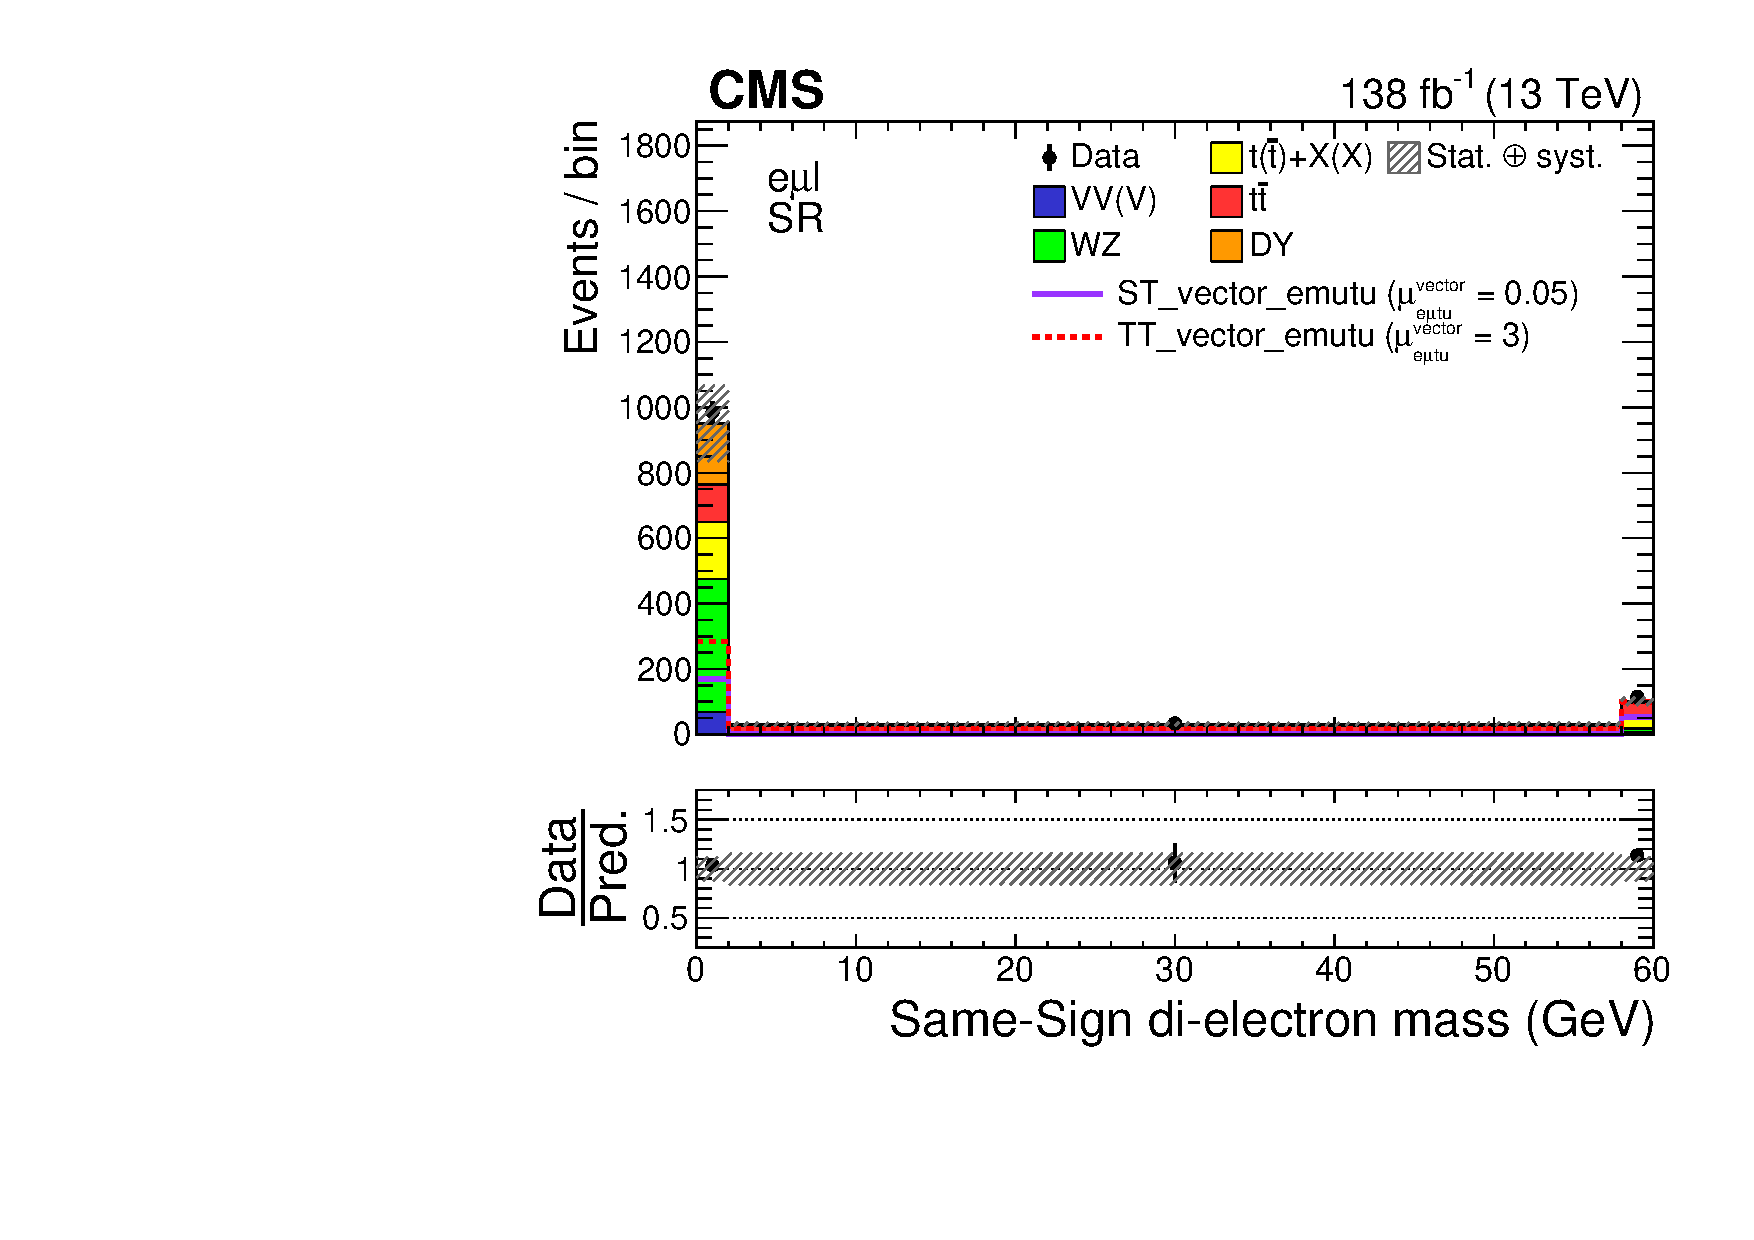
\includegraphics[width=0.325\textwidth]{figures/Appendix/SRMC/SSZmass}&
    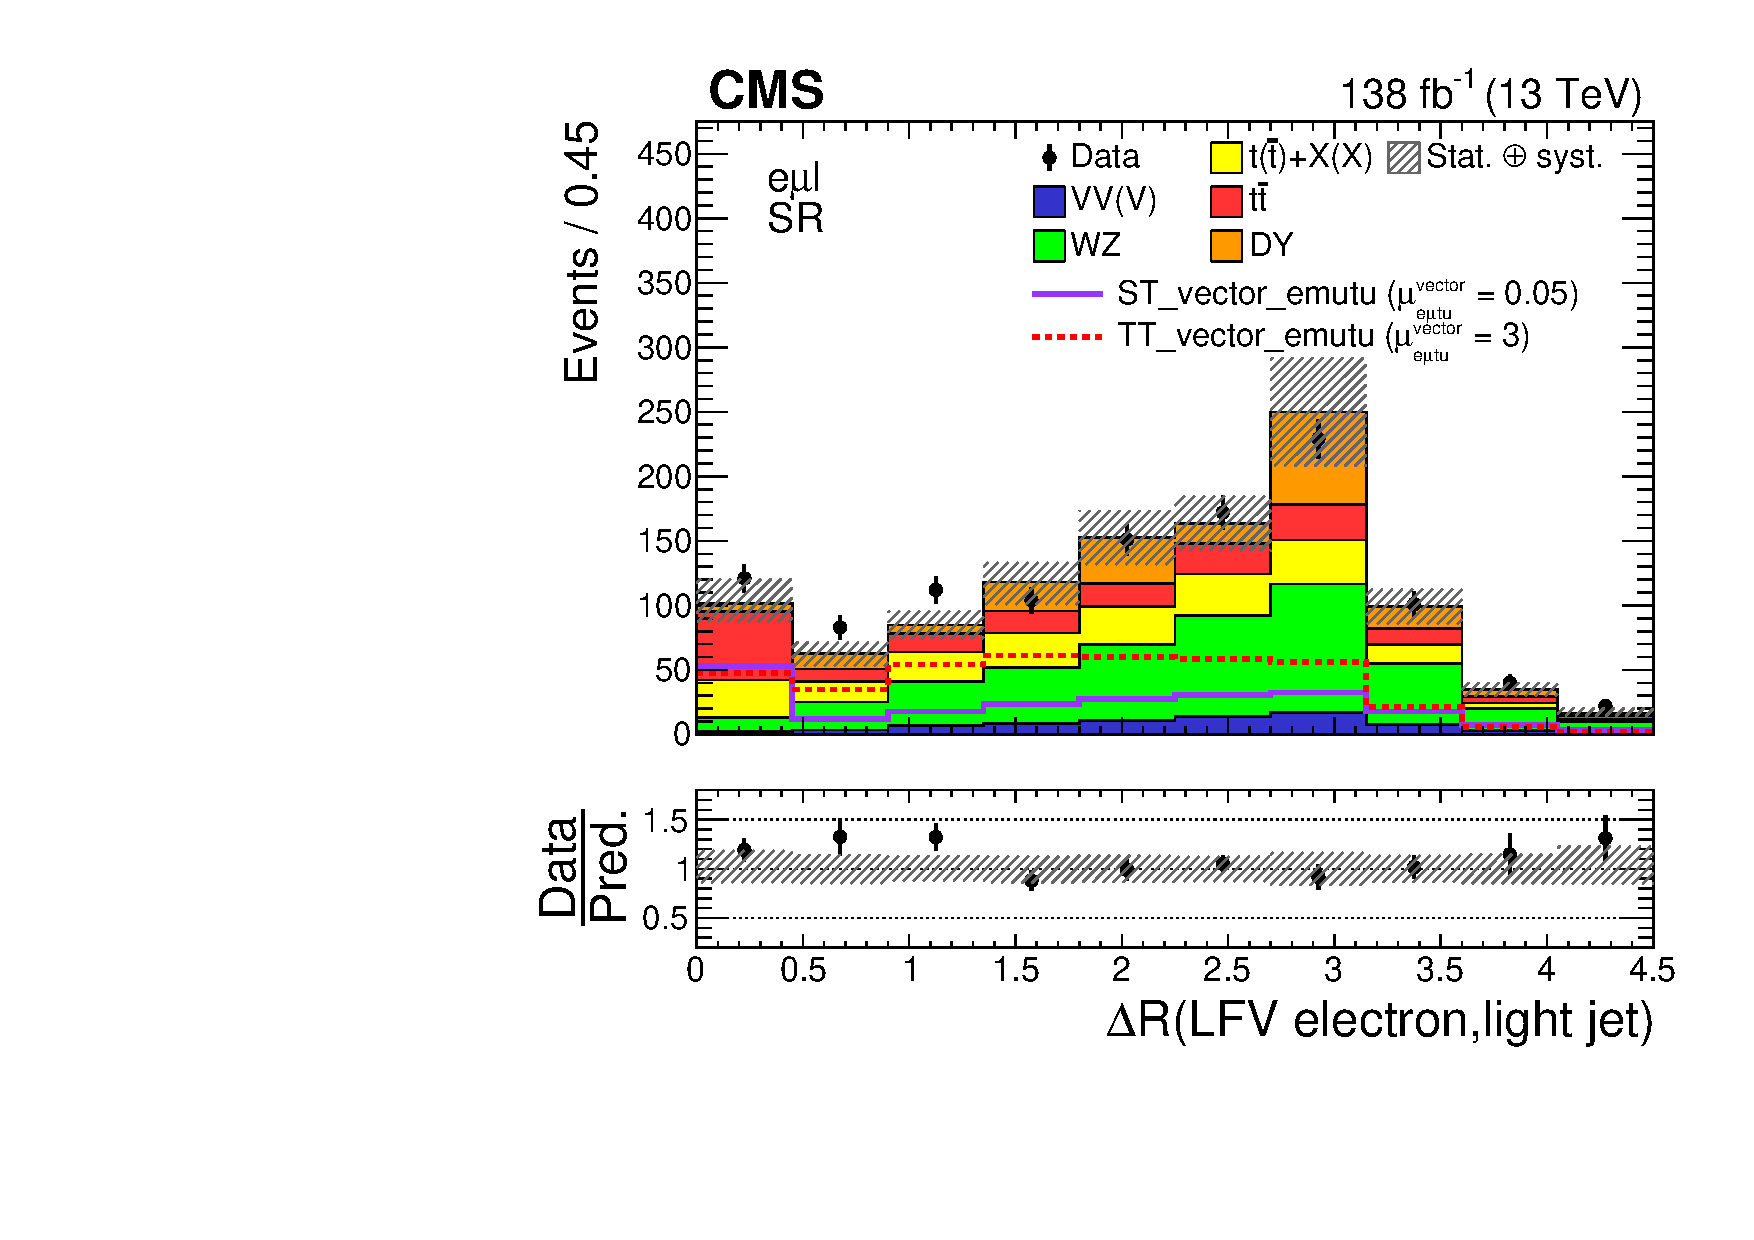
\includegraphics[width=0.325\textwidth]{figures/Appendix/SRMC/JeDr}&
  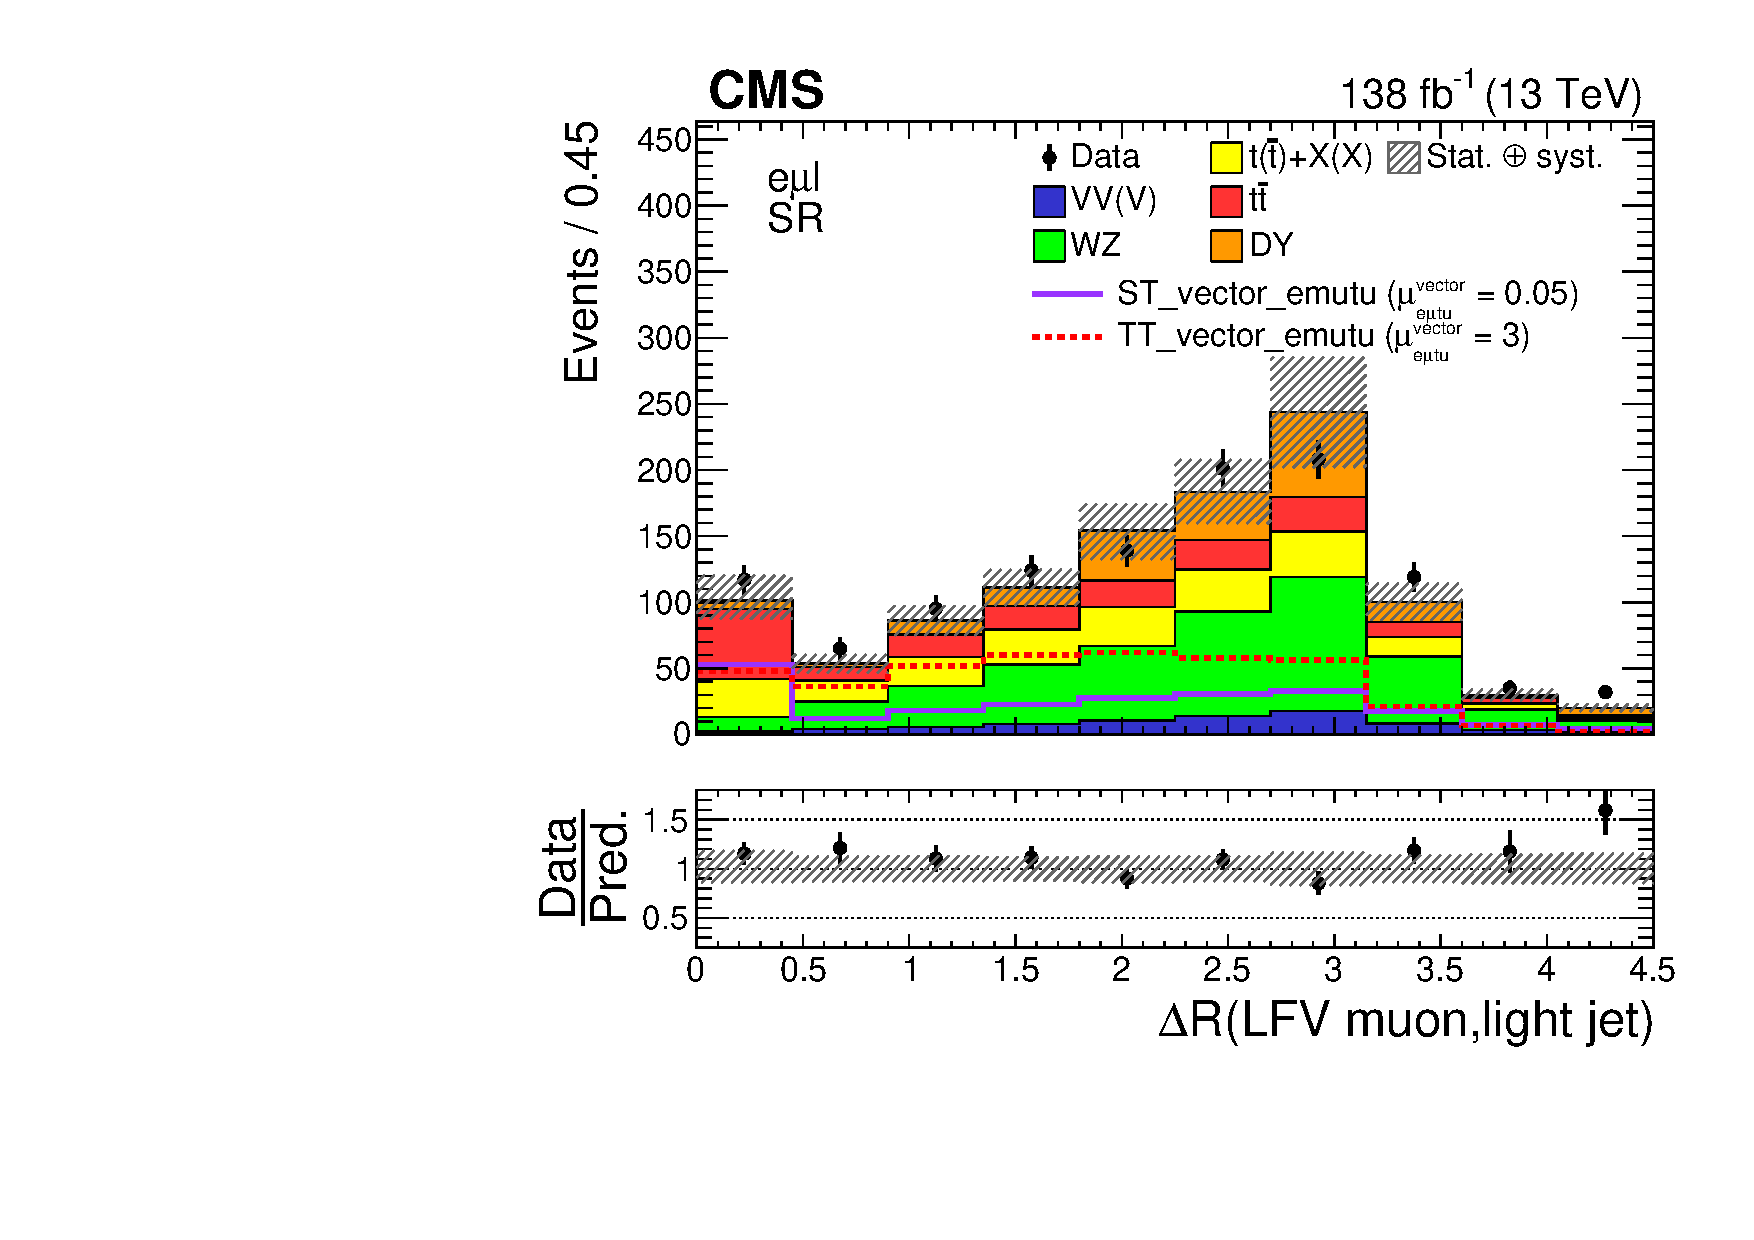
\includegraphics[width=0.325\textwidth]{figures/Appendix/SRMC/JmuDr}\\
 \end{tabular}
 \caption{Distributions of the same-sign di-electron mass (left), the opening angle between LFV electron and a light flavor jet (middle), and the opening angle between LFV muon and a light flavor jet (right).}
 \label{fig:input_vali_5}
 \end{center}
\end{figure}

\begin{figure}[tbh!]
 \begin{center}
 \begin{tabular}{ccc}
  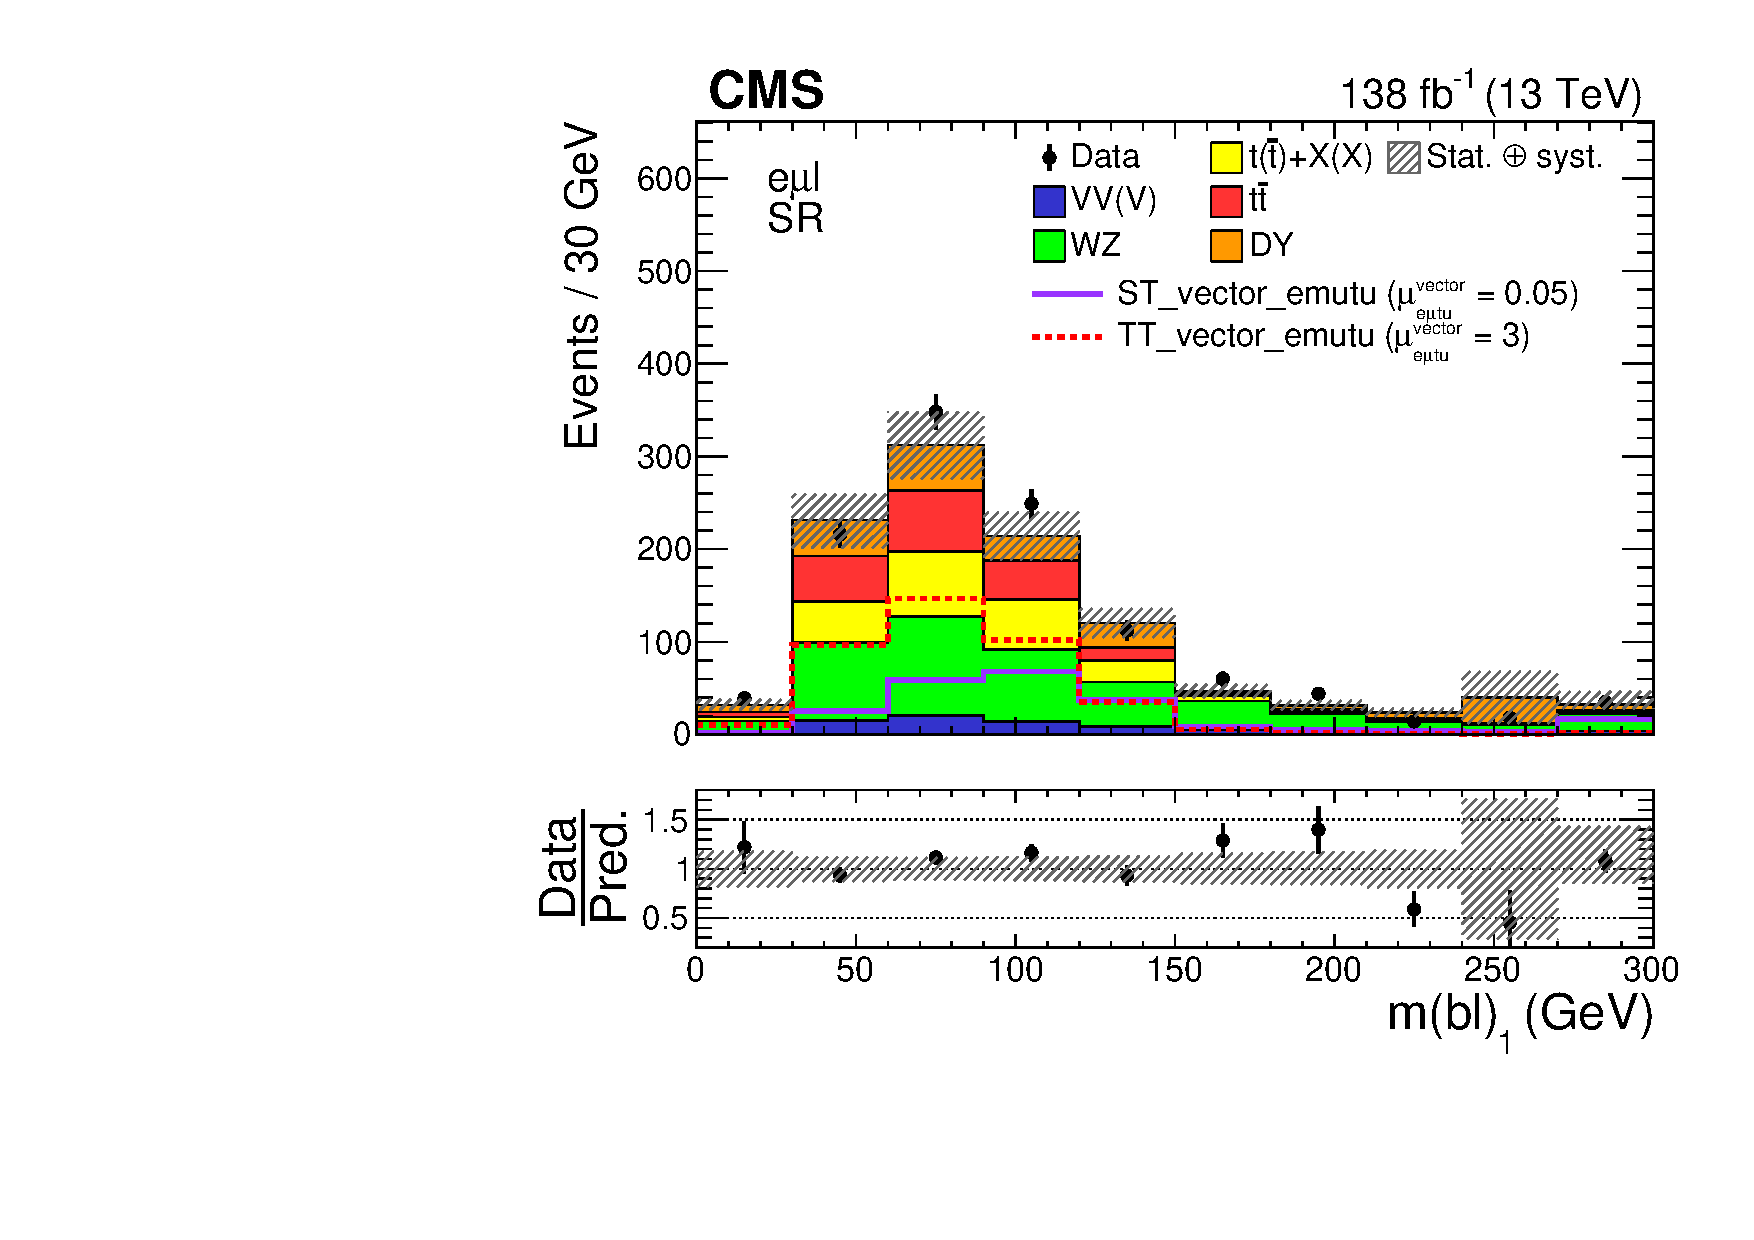
\includegraphics[width=0.325\textwidth]{figures/Appendix/SRMC/Mbl1}&
    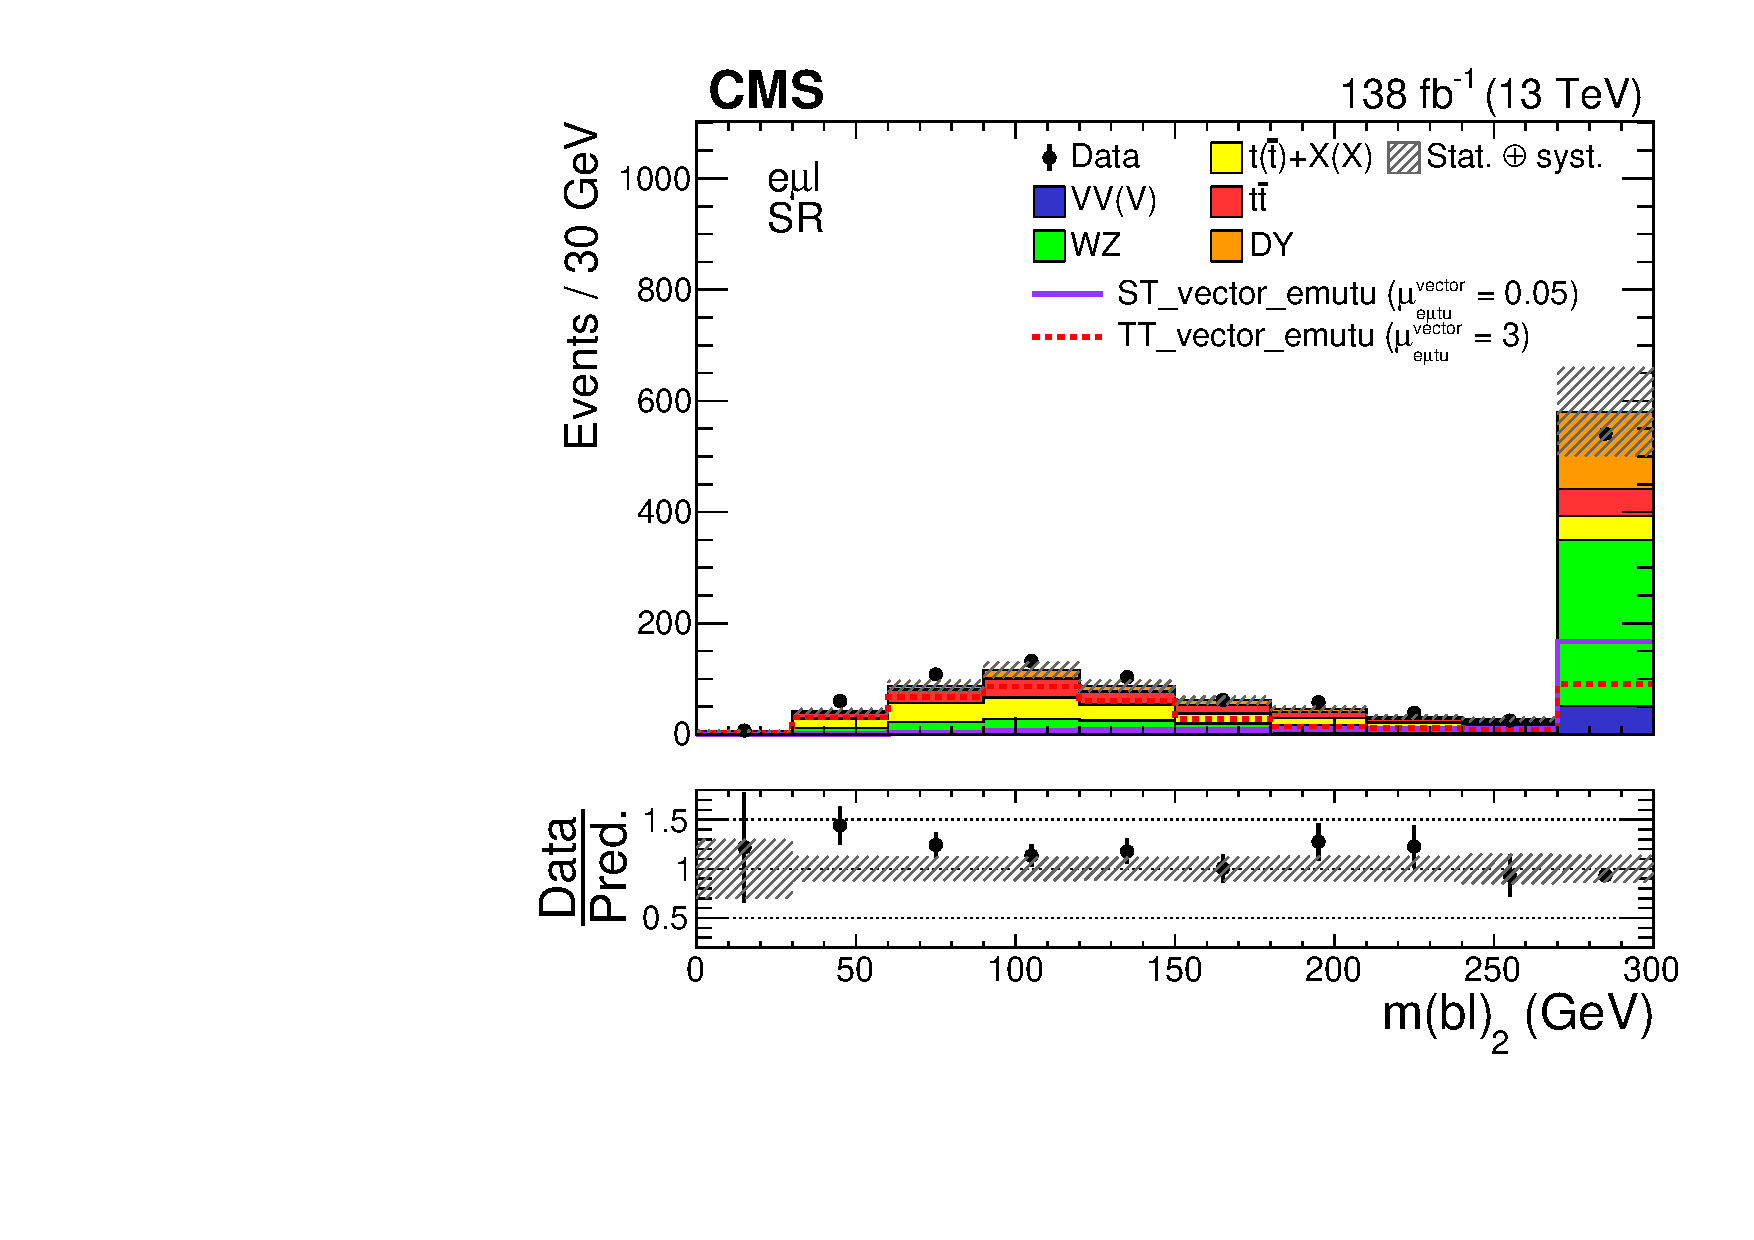
\includegraphics[width=0.325\textwidth]{figures/Appendix/SRMC/Mbl2}&
  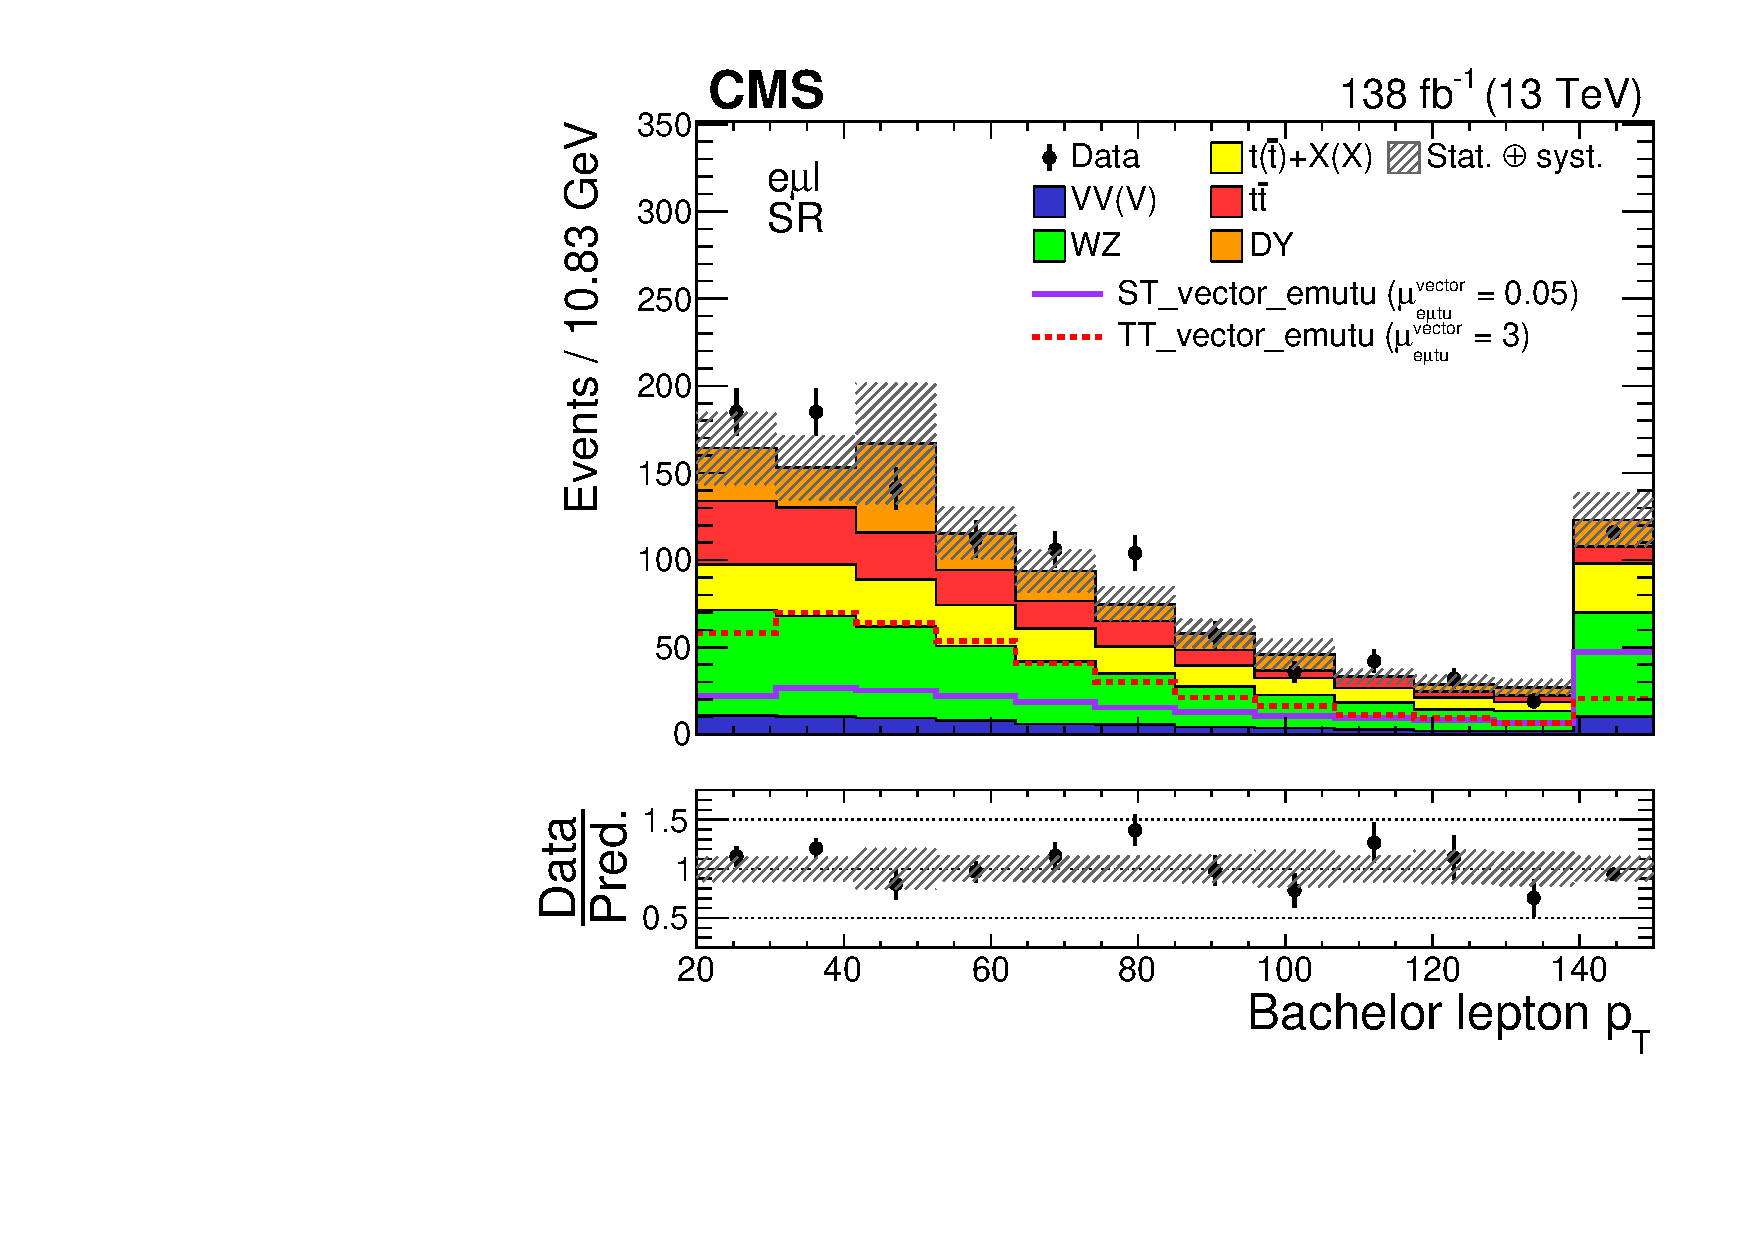
\includegraphics[width=0.325\textwidth]{figures/Appendix/SRMC/BaPt}\\
 \end{tabular}
 \caption{Distributions of the mass of the first $\mbl$ system (left), the mass of the second $\mbl$ system (middle), and standalone lepton $\pt$ (right).}
 \label{fig:input_vali_6}
 \end{center}
\end{figure}